\documentclass[12pt,a4paper]{article}

\usepackage[a4paper,text={16.5cm,25.2cm},centering]{geometry}
\usepackage{lmodern}
\usepackage{amssymb,amsmath}
\usepackage{bm}
\usepackage{graphicx}
\usepackage{microtype}
\usepackage{hyperref}
\setlength{\parindent}{0pt}
\setlength{\parskip}{1.2ex}

\hypersetup
       {   pdfauthor = {  },
           pdftitle={  },
           colorlinks=TRUE,
           linkcolor=black,
           citecolor=blue,
           urlcolor=blue
       }




\usepackage{upquote}
\usepackage{listings}
\usepackage{xcolor}
\lstset{
    basicstyle=\ttfamily\footnotesize,
    upquote=true,
    breaklines=true,
    breakindent=0pt,
    keepspaces=true,
    showspaces=false,
    columns=fullflexible,
    showtabs=false,
    showstringspaces=false,
    escapeinside={(*@}{@*)},
    extendedchars=true,
}
\newcommand{\HLJLt}[1]{#1}
\newcommand{\HLJLw}[1]{#1}
\newcommand{\HLJLe}[1]{#1}
\newcommand{\HLJLeB}[1]{#1}
\newcommand{\HLJLo}[1]{#1}
\newcommand{\HLJLk}[1]{\textcolor[RGB]{148,91,176}{\textbf{#1}}}
\newcommand{\HLJLkc}[1]{\textcolor[RGB]{59,151,46}{\textit{#1}}}
\newcommand{\HLJLkd}[1]{\textcolor[RGB]{214,102,97}{\textit{#1}}}
\newcommand{\HLJLkn}[1]{\textcolor[RGB]{148,91,176}{\textbf{#1}}}
\newcommand{\HLJLkp}[1]{\textcolor[RGB]{148,91,176}{\textbf{#1}}}
\newcommand{\HLJLkr}[1]{\textcolor[RGB]{148,91,176}{\textbf{#1}}}
\newcommand{\HLJLkt}[1]{\textcolor[RGB]{148,91,176}{\textbf{#1}}}
\newcommand{\HLJLn}[1]{#1}
\newcommand{\HLJLna}[1]{#1}
\newcommand{\HLJLnb}[1]{#1}
\newcommand{\HLJLnbp}[1]{#1}
\newcommand{\HLJLnc}[1]{#1}
\newcommand{\HLJLncB}[1]{#1}
\newcommand{\HLJLnd}[1]{\textcolor[RGB]{214,102,97}{#1}}
\newcommand{\HLJLne}[1]{#1}
\newcommand{\HLJLneB}[1]{#1}
\newcommand{\HLJLnf}[1]{\textcolor[RGB]{66,102,213}{#1}}
\newcommand{\HLJLnfm}[1]{\textcolor[RGB]{66,102,213}{#1}}
\newcommand{\HLJLnp}[1]{#1}
\newcommand{\HLJLnl}[1]{#1}
\newcommand{\HLJLnn}[1]{#1}
\newcommand{\HLJLno}[1]{#1}
\newcommand{\HLJLnt}[1]{#1}
\newcommand{\HLJLnv}[1]{#1}
\newcommand{\HLJLnvc}[1]{#1}
\newcommand{\HLJLnvg}[1]{#1}
\newcommand{\HLJLnvi}[1]{#1}
\newcommand{\HLJLnvm}[1]{#1}
\newcommand{\HLJLl}[1]{#1}
\newcommand{\HLJLld}[1]{\textcolor[RGB]{148,91,176}{\textit{#1}}}
\newcommand{\HLJLs}[1]{\textcolor[RGB]{201,61,57}{#1}}
\newcommand{\HLJLsa}[1]{\textcolor[RGB]{201,61,57}{#1}}
\newcommand{\HLJLsb}[1]{\textcolor[RGB]{201,61,57}{#1}}
\newcommand{\HLJLsc}[1]{\textcolor[RGB]{201,61,57}{#1}}
\newcommand{\HLJLsd}[1]{\textcolor[RGB]{201,61,57}{#1}}
\newcommand{\HLJLsdB}[1]{\textcolor[RGB]{201,61,57}{#1}}
\newcommand{\HLJLsdC}[1]{\textcolor[RGB]{201,61,57}{#1}}
\newcommand{\HLJLse}[1]{\textcolor[RGB]{59,151,46}{#1}}
\newcommand{\HLJLsh}[1]{\textcolor[RGB]{201,61,57}{#1}}
\newcommand{\HLJLsi}[1]{#1}
\newcommand{\HLJLso}[1]{\textcolor[RGB]{201,61,57}{#1}}
\newcommand{\HLJLsr}[1]{\textcolor[RGB]{201,61,57}{#1}}
\newcommand{\HLJLss}[1]{\textcolor[RGB]{201,61,57}{#1}}
\newcommand{\HLJLssB}[1]{\textcolor[RGB]{201,61,57}{#1}}
\newcommand{\HLJLnB}[1]{\textcolor[RGB]{59,151,46}{#1}}
\newcommand{\HLJLnbB}[1]{\textcolor[RGB]{59,151,46}{#1}}
\newcommand{\HLJLnfB}[1]{\textcolor[RGB]{59,151,46}{#1}}
\newcommand{\HLJLnh}[1]{\textcolor[RGB]{59,151,46}{#1}}
\newcommand{\HLJLni}[1]{\textcolor[RGB]{59,151,46}{#1}}
\newcommand{\HLJLnil}[1]{\textcolor[RGB]{59,151,46}{#1}}
\newcommand{\HLJLnoB}[1]{\textcolor[RGB]{59,151,46}{#1}}
\newcommand{\HLJLoB}[1]{\textcolor[RGB]{102,102,102}{\textbf{#1}}}
\newcommand{\HLJLow}[1]{\textcolor[RGB]{102,102,102}{\textbf{#1}}}
\newcommand{\HLJLp}[1]{#1}
\newcommand{\HLJLc}[1]{\textcolor[RGB]{153,153,119}{\textit{#1}}}
\newcommand{\HLJLch}[1]{\textcolor[RGB]{153,153,119}{\textit{#1}}}
\newcommand{\HLJLcm}[1]{\textcolor[RGB]{153,153,119}{\textit{#1}}}
\newcommand{\HLJLcp}[1]{\textcolor[RGB]{153,153,119}{\textit{#1}}}
\newcommand{\HLJLcpB}[1]{\textcolor[RGB]{153,153,119}{\textit{#1}}}
\newcommand{\HLJLcs}[1]{\textcolor[RGB]{153,153,119}{\textit{#1}}}
\newcommand{\HLJLcsB}[1]{\textcolor[RGB]{153,153,119}{\textit{#1}}}
\newcommand{\HLJLg}[1]{#1}
\newcommand{\HLJLgd}[1]{#1}
\newcommand{\HLJLge}[1]{#1}
\newcommand{\HLJLgeB}[1]{#1}
\newcommand{\HLJLgh}[1]{#1}
\newcommand{\HLJLgi}[1]{#1}
\newcommand{\HLJLgo}[1]{#1}
\newcommand{\HLJLgp}[1]{#1}
\newcommand{\HLJLgs}[1]{#1}
\newcommand{\HLJLgsB}[1]{#1}
\newcommand{\HLJLgt}[1]{#1}


\begin{document}



\section{Writing}
By Jojo Aboaf and Marty Wells

I am a visual human. Lets begin!


\begin{lstlisting}
(*@\HLJLk{using}@*) (*@\HLJLn{GRUtils}@*)
(*@\HLJLk{using}@*) (*@\HLJLn{StatsBase}@*)
\end{lstlisting}


\section{Abstract}
\begin{itemize}
\item We Construct a general methods to analyze permutations.


\item We present an empirical method for analyzing ordered in order to test for nationality bias in International Surf Competitions.


\item We show this method can be applied in other settings, particularly for random graphs.

\end{itemize}

To state what we are setting out to do in its full generality simply:

\begin{itemize}
\item We are interested in a (finite) set of things, $E = \{e_1, e_2, \dots, e_d \}$


\item The number of things we are interested in is $|E|=d$


\item We observe some data, $Y = (y_i)_i^N$


\item Each data point provides some information about a subset $\{e_a, e_b,\ensuremath{\ldots}, e_c \} \ensuremath{\subseteq} E$.


\item The number of things we observe is $|\{e_a, e_b,\ensuremath{\ldots}, e_c \} | = k$


\item We can observe

\begin{itemize}
\item a full ordering, for example $[e_c \:  e_a \ensuremath{\ldots} e_b]$


\item or a partial ordering, for example $[e_c \: \{e_a, \ensuremath{\ldots}, e_b\}]$, equivalently $[e_c \: \{e_b, \ensuremath{\ldots}, e_a\}]$


\item or no ordering at all.

\end{itemize}
\end{itemize}
\subsection{Concrete}
Does nationality influence the World Surf League Championship Tour? If so, how?, to what degree?, and does this vary depending on nationality?

\textbf{Ordered Data}: Recommendation systems attempt to leverage information regarding one\ensuremath{\rq}s preferences to suggest new content (e.g. music, movies) or products (e.g. books). Ranked-choice voting is used for local, provincial/state, and national level elections across the globe. Many institutions, such as Cornell University, use ranked-choice for its elections. In sports, team or athlete rankings frequently determine season schedules or tournament structures. And in games or general forms of competition, outcomes can be naturally expressed as an ordering of the set of participants.

\textbf{Graphical Data}: Graphs are everywhere and everyone loves graphs and so on...

\section{Introduction}
The World Surf League (WSL) is the most prominent organizer of international surf compeitions. Each year the WSL organizes a variety of "tours" which include Mens and Womens versions of Big Wave events, the "Longboard Tour", the "Qualifying Series", and the "Championship Tour" (CT). 

\subsection{Format}
Each year, the 32 highest ranked (shortboard) surfers are invited to participate in the "Championship Tour" (CT), which constists of 11 surf compeitions in 7 different countries. Each competition has 7 rounds, each consisting of 1 to 16 heats, and each heat has 2 to 3 surfers. Within a heat, a surfer may attempt to ride any number of waves, but their final heat score is the sum of their two highest scoring waves. The surfer with the highest heat score places 1st in the heat, the surfer with the next highest heat score places 2nd in the heat. In some rounds, heats consist of 3 surfers, in which case the surfer with the third highest heat score will place 3rd in the heat. Each round has a rule that determines which surfers advance, and what (round,heat) they advance to. Surfers that do not advance "exit" the event, and are given some number of points (the closer the exit is to the compeitions final round, the higher the amount of points).

INSERT 2019 Event Format Drawing Here: Note to self: add number of points given at exit to fig.

\subsection{Data}

We collected some incredibly rich data on surf compeitions from the 2017, 2018, and 2019 seasons of the Mens World Championship Tour (WCT). Each year the World Surf League (WCT) holds 10 to 11 surf competitions, which are called "events". While the format of events have changed slightly between the 2017 and 2019 seasons, they are all very similar. Each event consists of 7 rounds, and within each round there are some number of heats. A heat is the level at which intra-athlete competition takes place and may consist of 2 or 3 surfers. Throughout a timed heat (usually between 22 and 35 minutes), each athlete may surf any number of waves and their "heat score" is the sum of the scores of their two highest scoring waves. 


Question: How are waves scored? In any given heat, there is judging panel comprised of 5 judges. Anytime a surfer attempts to ride a wave, each judge analyzes the surfer's ride with respect to the following criteria and write down a score:

\begin{itemize}
\item Commitment and degree of difficulty


\item Innovative and progressive maneuvers


\item Combination of major maneuvers


\item Variety of maneuvers


\item Speed, power, and flow

\end{itemize}
Note: that Different elements of this list may be emphasized more or less depending on the location, conditions, and changes of conditions. (Chapter 13 Article 182) Additionally, the General Judging Rules (Chapter 13; Article 183; Section 1,2) state that judges should be visually separated, should not discuss scores, and may not change their scores.


Though there are 5 judges and 5 scores, the score a surfer receives, called the "wave score", is the trimmed mean of the scores given by the 5 judges. This is very important information and particularly interesting because it distinguishes the \emph{existence} of biased judges from the effect of biased judging (if it exists).


However, there are some intricacies. The judging process does not only consist of 5 judges. For each mens CT event, there is 1 international Head Judge, 7 international judges, and 1 international priority Judge (Chapter 13, Article 179.01). And Chapter 13, article 179.17 states that "At CT Events, the number of judges from any one regional area is limited to 3". For each heat, the WSL Head Judge must assure there are at least 5 judges on the panel for each heat and that they are a subset of the 7 International Judges and 1 International Head Judge (Chapter 13, Article 179.13).


5 judges are selected from a pool of 8 judges to form a panel for a heat. During that heat, when a surfer rides a wave, each judge independently observes the ride and writes down a score (based on some broadly defined criteria), which is some number in \{0.0, 0.1, 0.2, ..., 9.8, 9.9, 10.0\}.


\subsection{Judging Panel Data}
Question: What is the definition of a panel? What type of data is it? For any given heat, there are 5 judges on the judging panel. Anytime a surfer rides a wave, each of them observes the way 

What does a panel look like? A lot of very different things that may seem very similar BUT ARE NOT. For example:


\begin{lstlisting}
(*@\HLJLnf{include}@*)(*@\HLJLp{(}@*)(*@\HLJLs{"{}EquivPanelData.jl"{}}@*)(*@\HLJLp{)}@*)
(*@\HLJLnf{display}@*)(*@\HLJLp{(}@*)(*@\HLJLn{eqPanels}@*)(*@\HLJLp{[}@*)(*@\HLJLni{1}@*)(*@\HLJLp{])}@*)
(*@\HLJLnf{display}@*)(*@\HLJLp{(}@*)(*@\HLJLn{eqPanels}@*)(*@\HLJLp{[}@*)(*@\HLJLni{3}@*)(*@\HLJLp{])}@*)
(*@\HLJLnf{display}@*)(*@\HLJLp{(}@*)(*@\HLJLn{eqPanels}@*)(*@\HLJLp{[}@*)(*@\HLJLni{5}@*)(*@\HLJLp{])}@*)
\end{lstlisting}

\begin{lstlisting}
1-element Array(*@{{\{}}@*)Pair,1(*@{{\}}}@*):
 Float16[3.5, 4.5, 4.0, 4.0, 4.0] => [:AUS, :AUS, :USA, :BRA, :BRA]
5-element Array(*@{{\{}}@*)Pair,1(*@{{\}}}@*):
 Float16[1.0] => [:BRA]
 Float16[1.1] => [:USA]
 Float16[1.2] => [:AUS]
 Float16[1.3] => [:PRT]
 Float16[1.5] => [:ESP]
4-element Array(*@{{\{}}@*)Pair,1(*@{{\}}}@*):
 Float16[0.5, 0.5] => [:ESP, :FRA]
      Float16[0.8] => [:AUS]
      Float16[1.0] => [:BRA]
      Float16[1.2] => [:USA]
\end{lstlisting}


\section{Motivation}
Our goal is to determine if judges have a tendency to give higher scores to surfers that share their same nationality.


The straight forward approach is to identify all of the "matching judges" for each wave, which are the judges scoring a surfer that have the same nationality as the surfer. 


Though we will use the term "matching judge(s)" throughout the paper, it is important to keep in mind that it is both the Athlete origin and Judge origin which determine if a judge is a "matching judge" or a "non-matching judge".


Some instinctual approaches:

\begin{itemize}
\item H\_0: Mean of matching judges = mean of non-matching judges

\begin{itemize}
\item This approach can work, but not always. It will fail if 

\end{itemize}
\end{itemize}

\begin{tabular}
{r | r | r | r | r | r | r | r}
Country & Judges (n) & Waves & Per Wave & Mean & SD & T-Value & P-Value \\
\hline
Australia & 4972 & 3250 & 1.529846 & 0.017198 & 0.351363 & 3.451332 & 0.000562 \\
Brazil & 8340 & 5234 & 1.593428 & 0.009411 & 0.330016 & 2.604384 & 0.009220 \\
France & 682 & 682 & 1 & 0.048167 & 0.320114 & 3.929514 & 0.000094 \\
French Polynesia & 10 & 10 & 1 & 0.010000 & 0.425617 & 0.074299 & 0.942398 \\
Hawaii & 122 & 122 & 1 & 0.024795 & 0.298571 & 0.917272 & 0.360825 \\
Portugal & 203 & 203 & 1 & 0.021552 & 0.358535 & 0.856443 & 0.392767 \\
South Africa & 257 & 257 & 1 & 0.044261 & 0.341772 & 2.076101 & 0.038883 \\
United States & 1277 & 1131 & 1.129089 & 0.026625 & 0.329370 & 2.888684 & 0.003934 \\
\end{tabular}

\section{Methods}
\subsection{Lets explore the Data!}
We have lots of missing Judge Origins from panels in the 2017 World Surf League season so we will omit the 2017 season ... for now (This begs an intersting question which we should return to later).


We have constructed a multidimensional array, aka an m-way, cross classified, contingency table. We have m classification factors:

\begin{itemize}
\item WSL Season


\item Event


\item Round


\item Heat


\item Ahtlete Origin


\item Judge Origin


\item Size of Partition of Panel (Max Rank)


\item Rank of Judge

\end{itemize}

\begin{lstlisting}
(*@\HLJLnf{include}@*)(*@\HLJLp{(}@*)(*@\HLJLs{"{}RankingTensor.jl"{}}@*)(*@\HLJLp{)}@*)
(*@\HLJLnf{println}@*)(*@\HLJLp{(}@*)(*@\HLJLs{"{}m}@*) (*@\HLJLs{=}@*) (*@\HLJLsi{{\$}}@*)(*@\HLJLp{(}@*)(*@\HLJLnf{ndims}@*)(*@\HLJLp{(}@*)(*@\HLJLn{info}@*)(*@\HLJLp{))}@*)(*@\HLJLs{"{}}@*)(*@\HLJLp{)}@*)
(*@\HLJLnf{println}@*)(*@\HLJLp{(}@*)(*@\HLJLnf{size}@*)(*@\HLJLp{(}@*)(*@\HLJLn{info}@*)(*@\HLJLp{))}@*)

(*@\HLJLk{function}@*) (*@\HLJLnf{marginalBarPlot}@*)(*@\HLJLp{(}@*)(*@\HLJLn{M}@*)(*@\HLJLoB{::}@*)(*@\HLJLnf{Array}@*)(*@\HLJLp{{\{}}@*)(*@\HLJLn{T}@*)(*@\HLJLp{,}@*)(*@\HLJLn{N}@*)(*@\HLJLp{{\}},}@*) (*@\HLJLn{d}@*)(*@\HLJLoB{::}@*)(*@\HLJLn{Integer}@*)(*@\HLJLp{)}@*) (*@\HLJLn{where}@*) (*@\HLJLp{{\{}}@*)(*@\HLJLn{T}@*)(*@\HLJLp{,}@*)(*@\HLJLn{N}@*)(*@\HLJLp{{\}}}@*)
	(*@\HLJLnf{dIndex{\_}}@*)(*@\HLJLp{(}@*)(*@\HLJLn{h}@*)(*@\HLJLoB{::}@*)(*@\HLJLn{Integer}@*)(*@\HLJLp{)}@*) (*@\HLJLoB{=}@*) (*@\HLJLp{[}@*) (*@\HLJLn{i}@*)(*@\HLJLoB{==}@*)(*@\HLJLn{d}@*) (*@\HLJLoB{?}@*) (*@\HLJLn{h}@*) (*@\HLJLoB{:}@*) (*@\HLJLnf{Colon}@*)(*@\HLJLp{()}@*) (*@\HLJLk{for}@*) (*@\HLJLn{i}@*) (*@\HLJLkp{in}@*) (*@\HLJLni{1}@*)(*@\HLJLoB{:}@*)(*@\HLJLn{N}@*)(*@\HLJLp{]}@*)
	(*@\HLJLn{marginal{\_}d}@*) (*@\HLJLoB{=}@*) (*@\HLJLp{[}@*)(*@\HLJLnf{sum}@*)(*@\HLJLp{(}@*) (*@\HLJLn{M}@*)(*@\HLJLp{[}@*) (*@\HLJLnf{dIndex{\_}}@*)(*@\HLJLp{(}@*)(*@\HLJLn{h}@*)(*@\HLJLp{)}@*)(*@\HLJLoB{...}@*) (*@\HLJLp{]}@*) (*@\HLJLp{)}@*) (*@\HLJLk{for}@*) (*@\HLJLn{h}@*) (*@\HLJLkp{in}@*) (*@\HLJLni{1}@*)(*@\HLJLoB{:}@*)(*@\HLJLnf{size}@*)(*@\HLJLp{(}@*)(*@\HLJLn{M}@*)(*@\HLJLp{)[}@*)(*@\HLJLn{d}@*)(*@\HLJLp{]}@*) (*@\HLJLp{]}@*)
	(*@\HLJLnf{savefig}@*)(*@\HLJLp{(}@*)
		(*@\HLJLs{"{}visuals/marginal{\_}}@*)(*@\HLJLsi{{\$}}@*)(*@\HLJLp{(}@*)(*@\HLJLn{vars}@*)(*@\HLJLp{[}@*)(*@\HLJLn{d}@*)(*@\HLJLp{])}@*)(*@\HLJLs{.png"{}}@*)(*@\HLJLp{,}@*)
		(*@\HLJLnf{barplot}@*)(*@\HLJLp{(}@*)
			(*@\HLJLnf{map}@*)(*@\HLJLp{(}@*)(*@\HLJLn{x}@*)(*@\HLJLoB{->}@*) (*@\HLJLs{"{}}@*)(*@\HLJLsi{{\$}}@*)(*@\HLJLp{(}@*)(*@\HLJLn{x}@*)(*@\HLJLp{)}@*)(*@\HLJLs{"{}}@*)(*@\HLJLp{,}@*) (*@\HLJLnf{sort}@*)(*@\HLJLp{(}@*)(*@\HLJLnf{collect}@*)(*@\HLJLp{(}@*)(*@\HLJLnf{keys}@*)(*@\HLJLp{(}@*)(*@\HLJLn{ToInd}@*)(*@\HLJLp{[}@*)(*@\HLJLn{vars}@*)(*@\HLJLp{[}@*)(*@\HLJLn{d}@*)(*@\HLJLp{]])))}@*) (*@\HLJLp{),}@*)
			(*@\HLJLn{marginal{\_}d}@*)
		(*@\HLJLp{)}@*)
	(*@\HLJLp{)}@*)
	(*@\HLJLk{return}@*) (*@\HLJLn{marginal{\_}d}@*)
(*@\HLJLk{end}@*)

(*@\HLJLk{for}@*) (*@\HLJLn{d}@*) (*@\HLJLkp{in}@*) (*@\HLJLnf{length}@*)(*@\HLJLp{(}@*)(*@\HLJLn{vars}@*)(*@\HLJLp{)}@*) (*@\HLJLnf{marginalBarPlot}@*)(*@\HLJLp{(}@*)(*@\HLJLn{info}@*)(*@\HLJLp{,}@*) (*@\HLJLn{d}@*)(*@\HLJLp{)}@*) (*@\HLJLk{end}@*)
\end{lstlisting}

\begin{lstlisting}
m = 8
(2, 10, 7, 16, 10, 7, 5, 5)
\end{lstlisting}


\begin{figure}
\centering
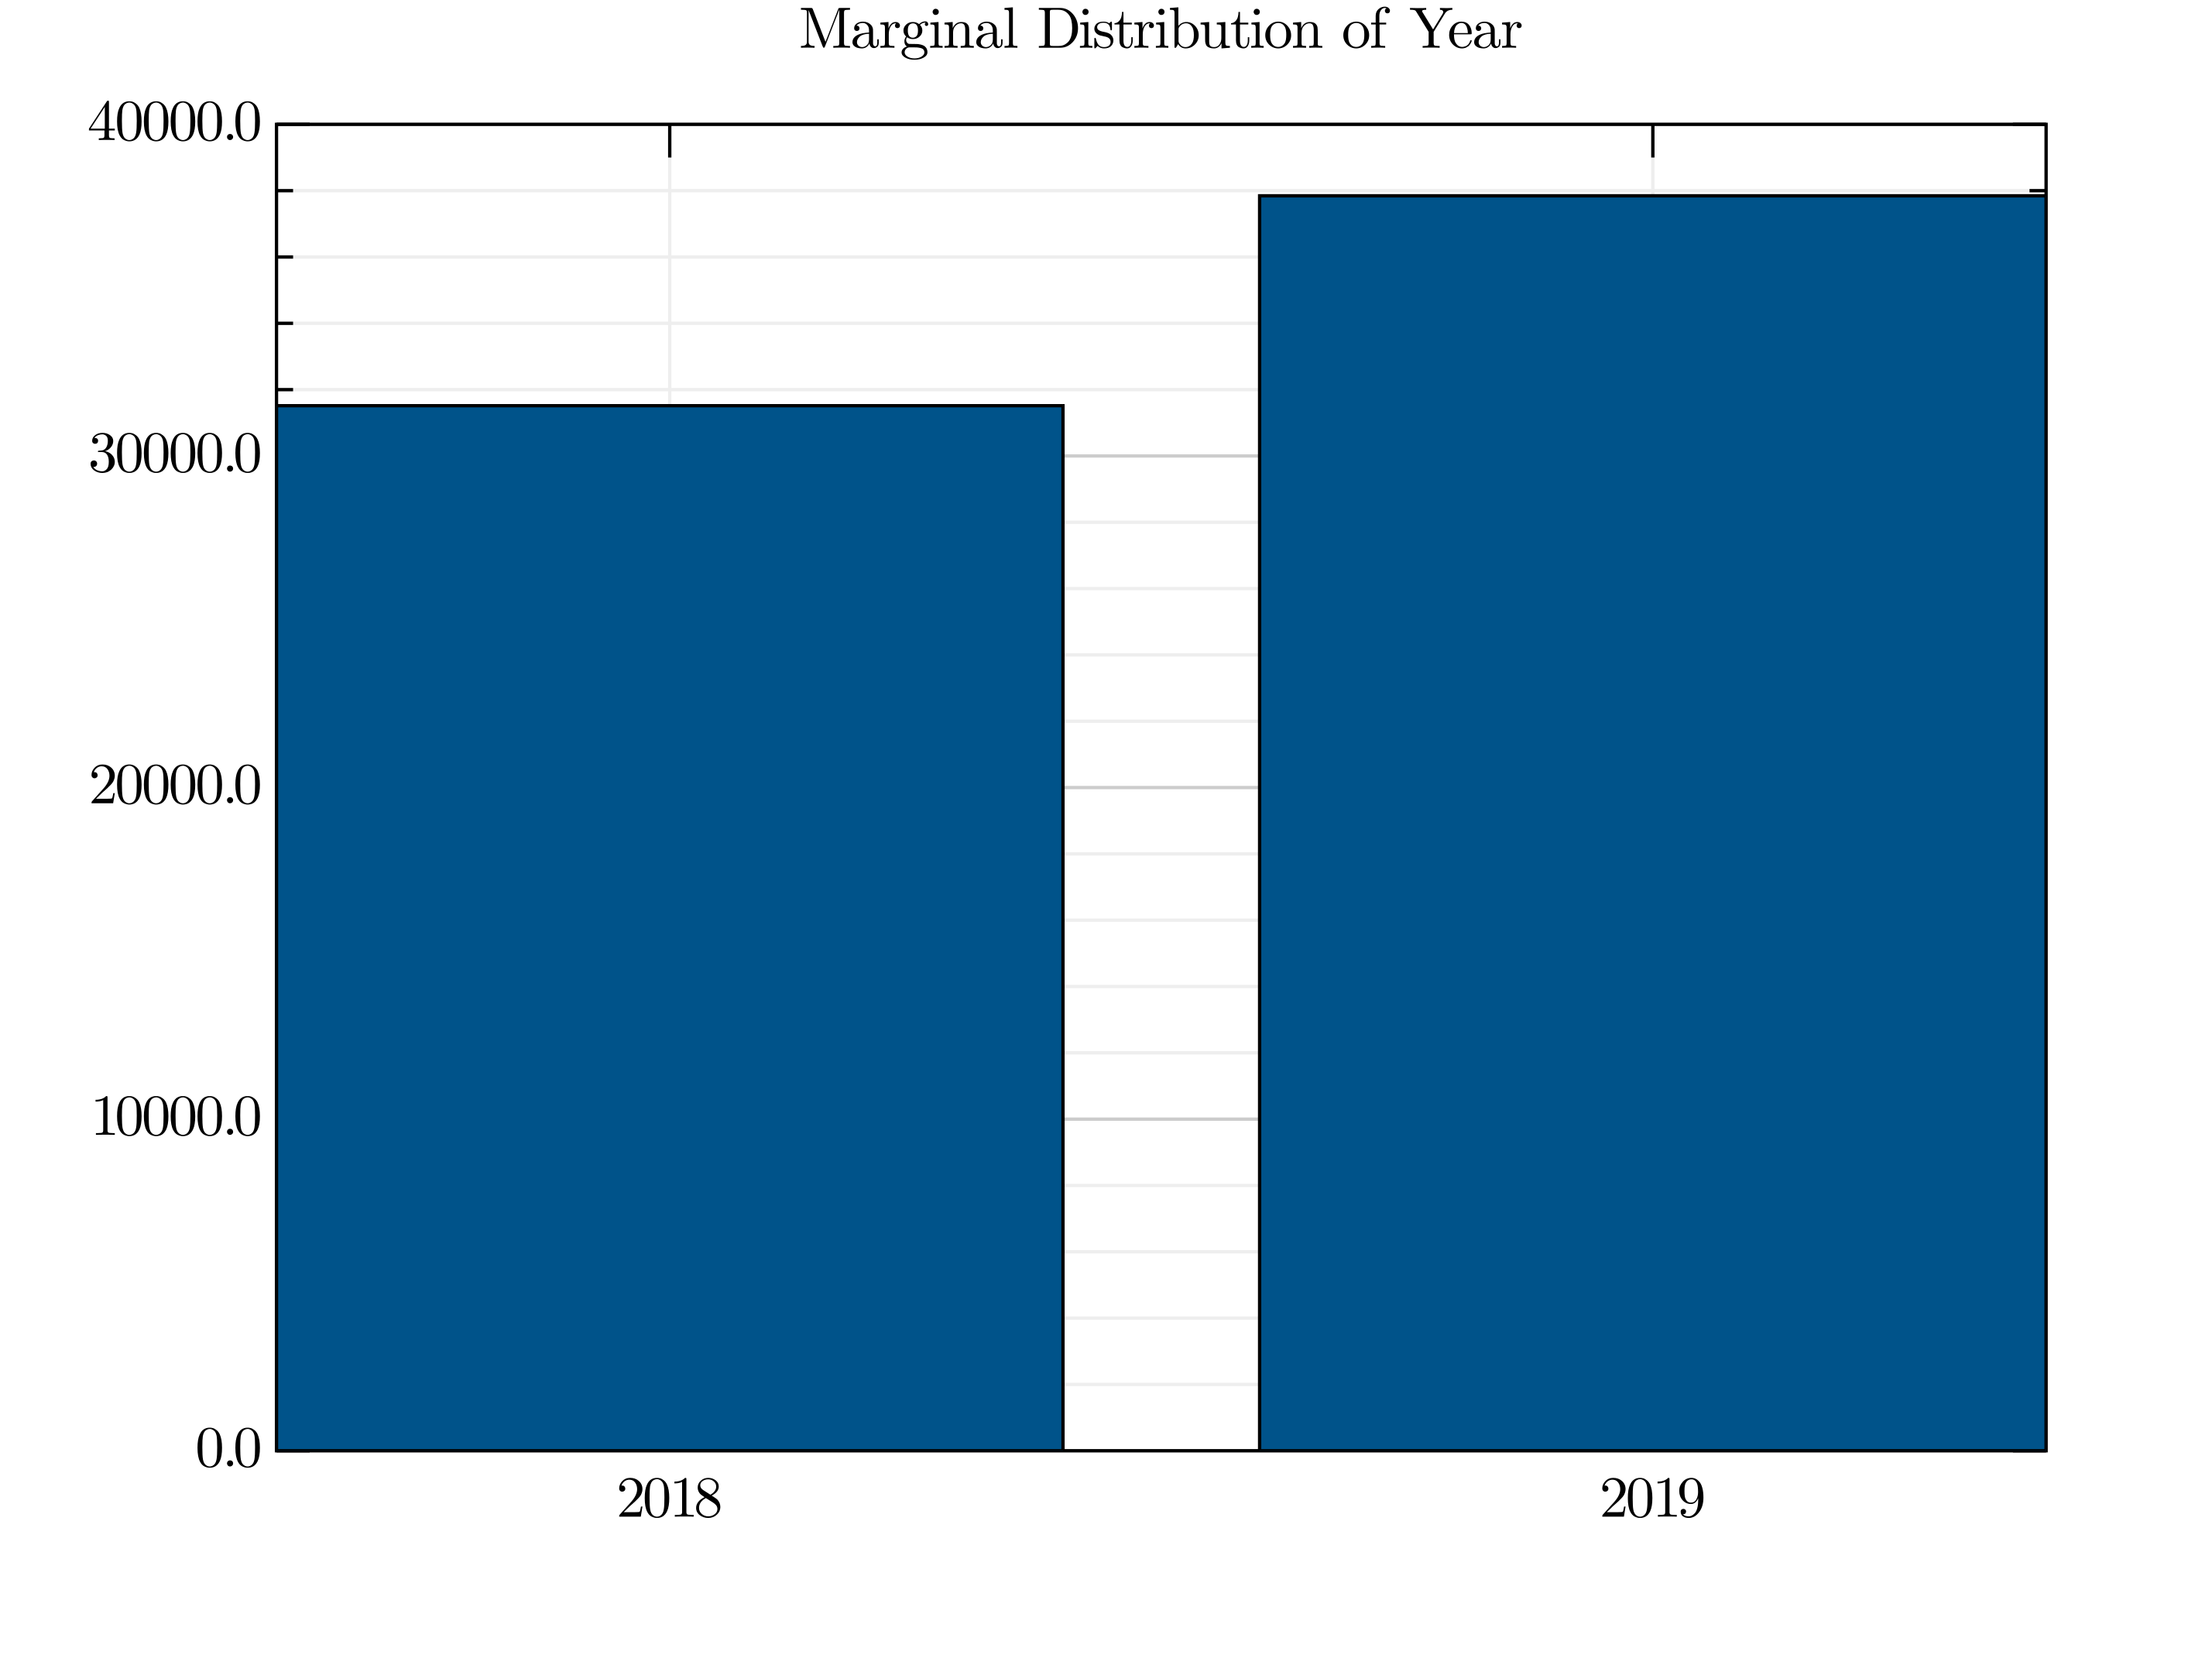
\includegraphics{visuals/marginals_YR.png}
\caption{Judge Origin Marginal}
\end{figure}
 \begin{figure}
\centering
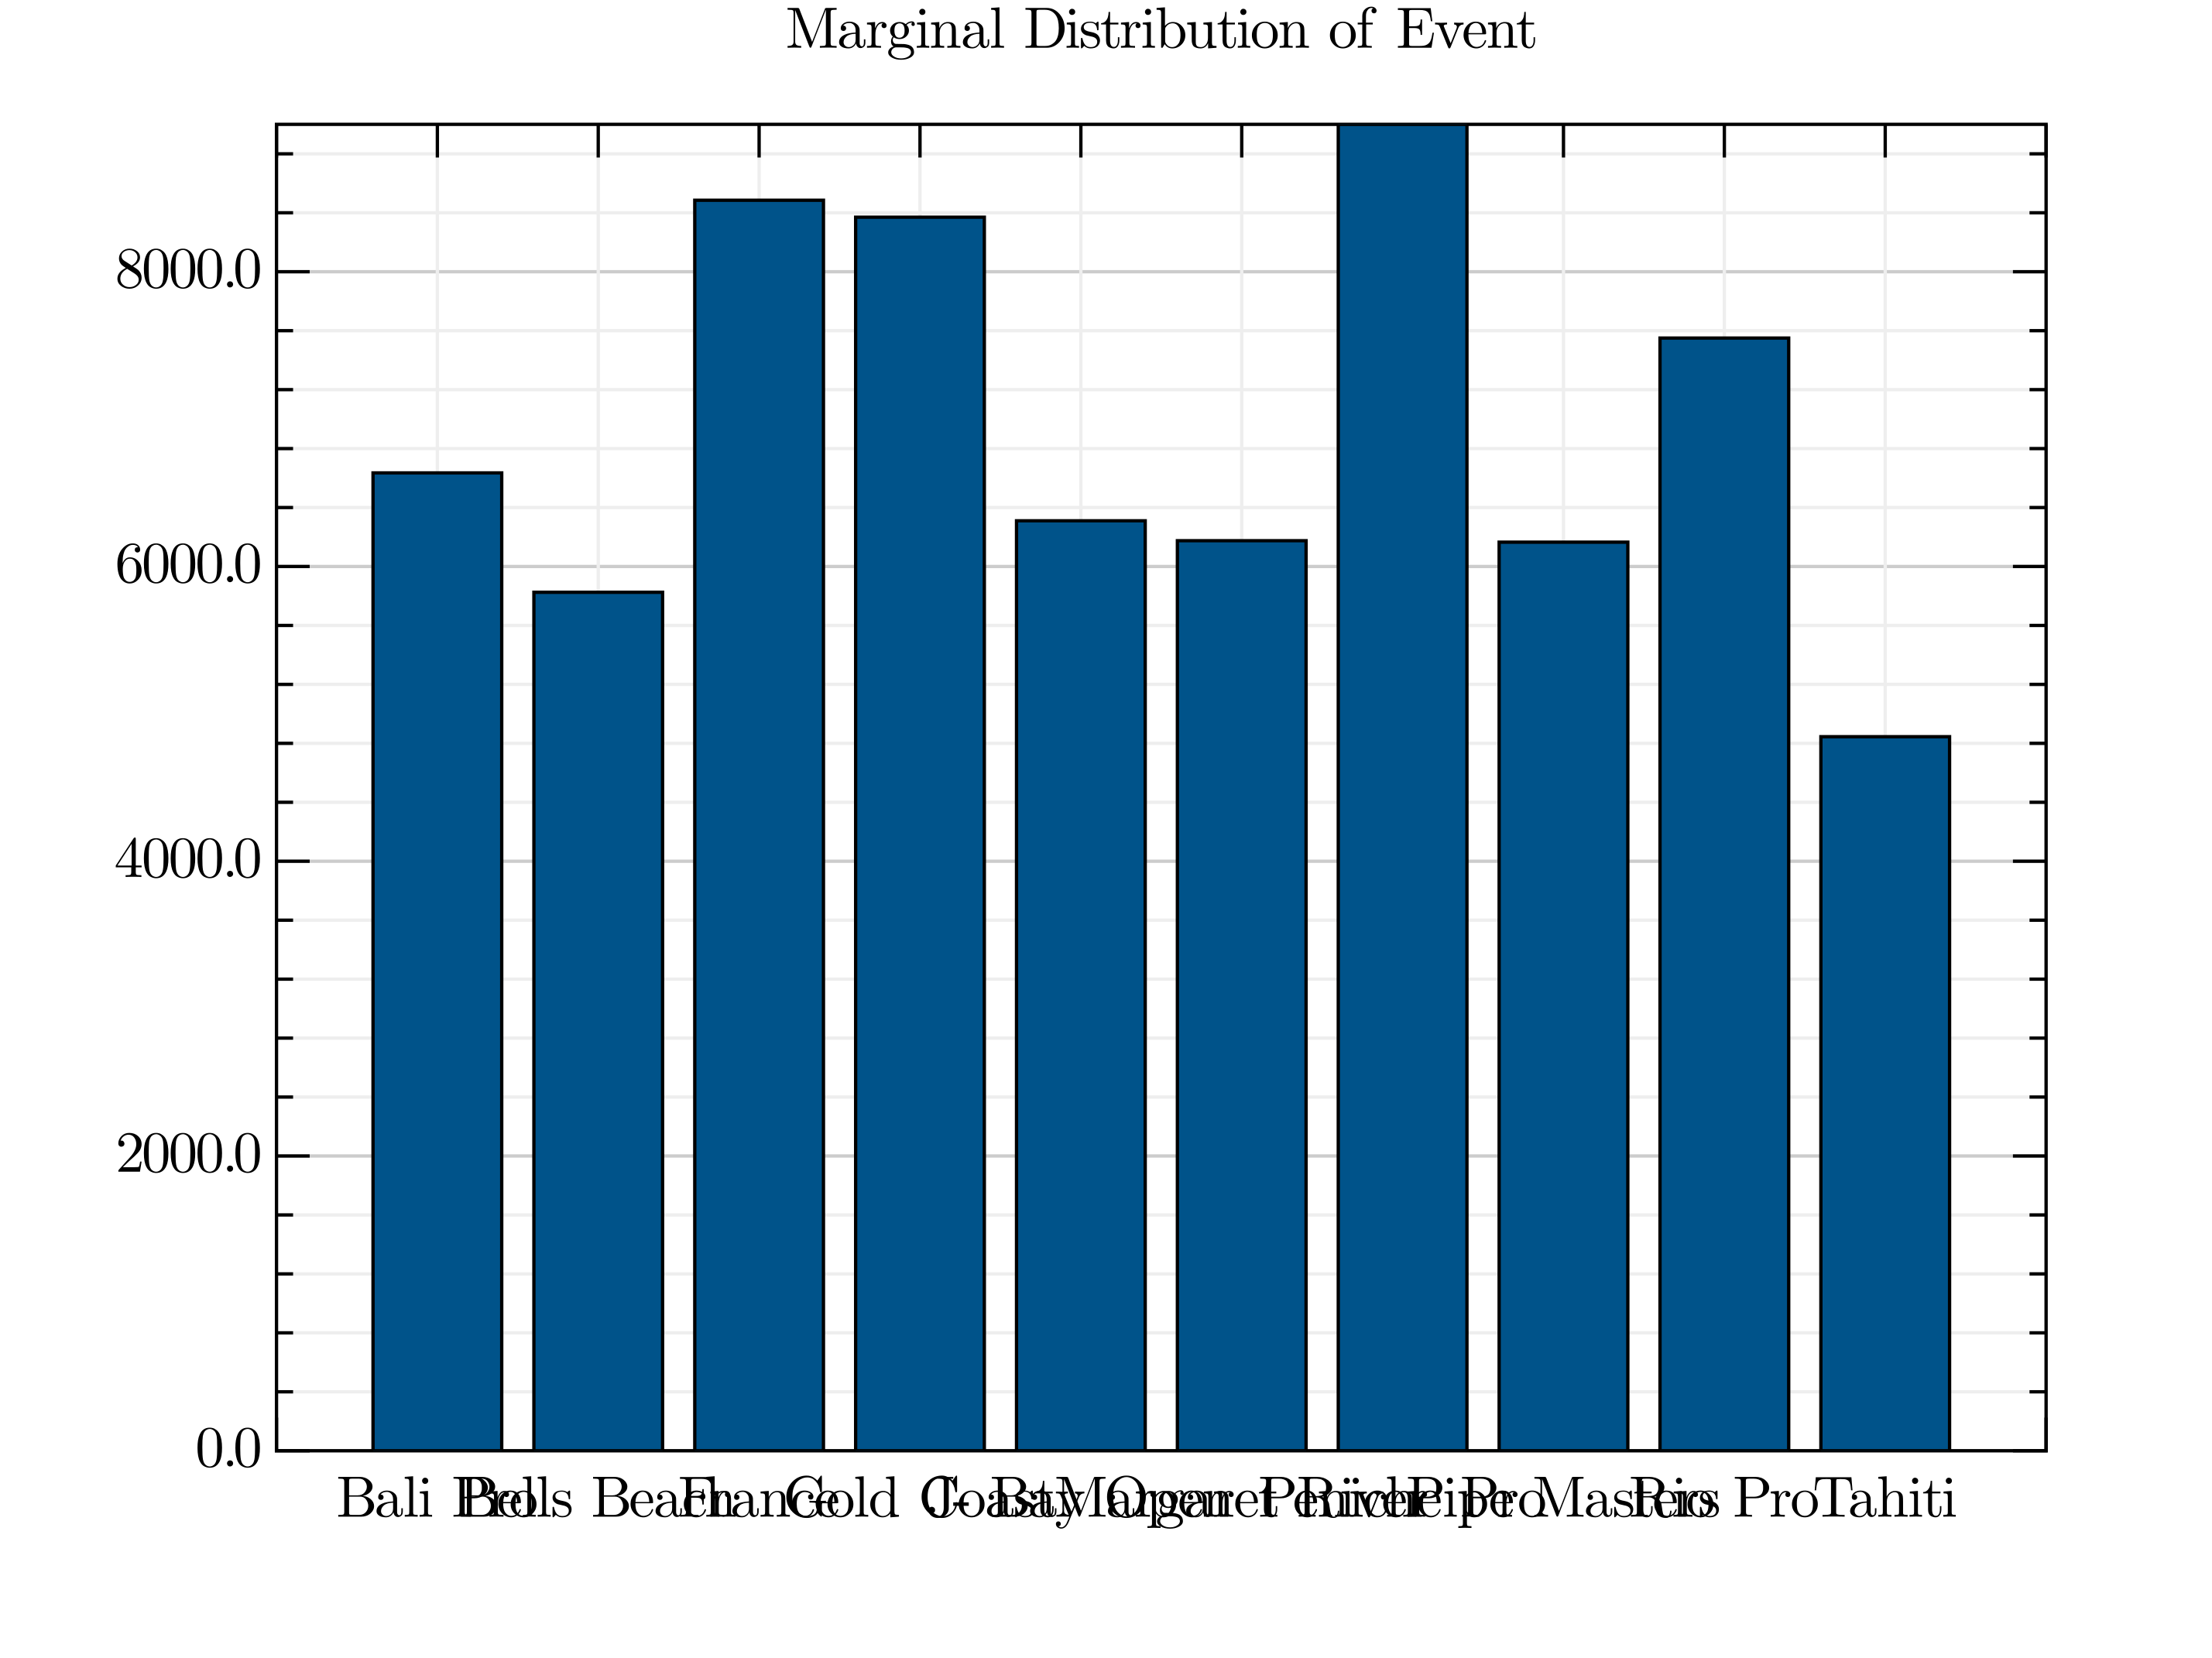
\includegraphics{visuals/marginals_EVT.png}
\caption{Judge Origin Marginal}
\end{figure}
 \begin{figure}
\centering
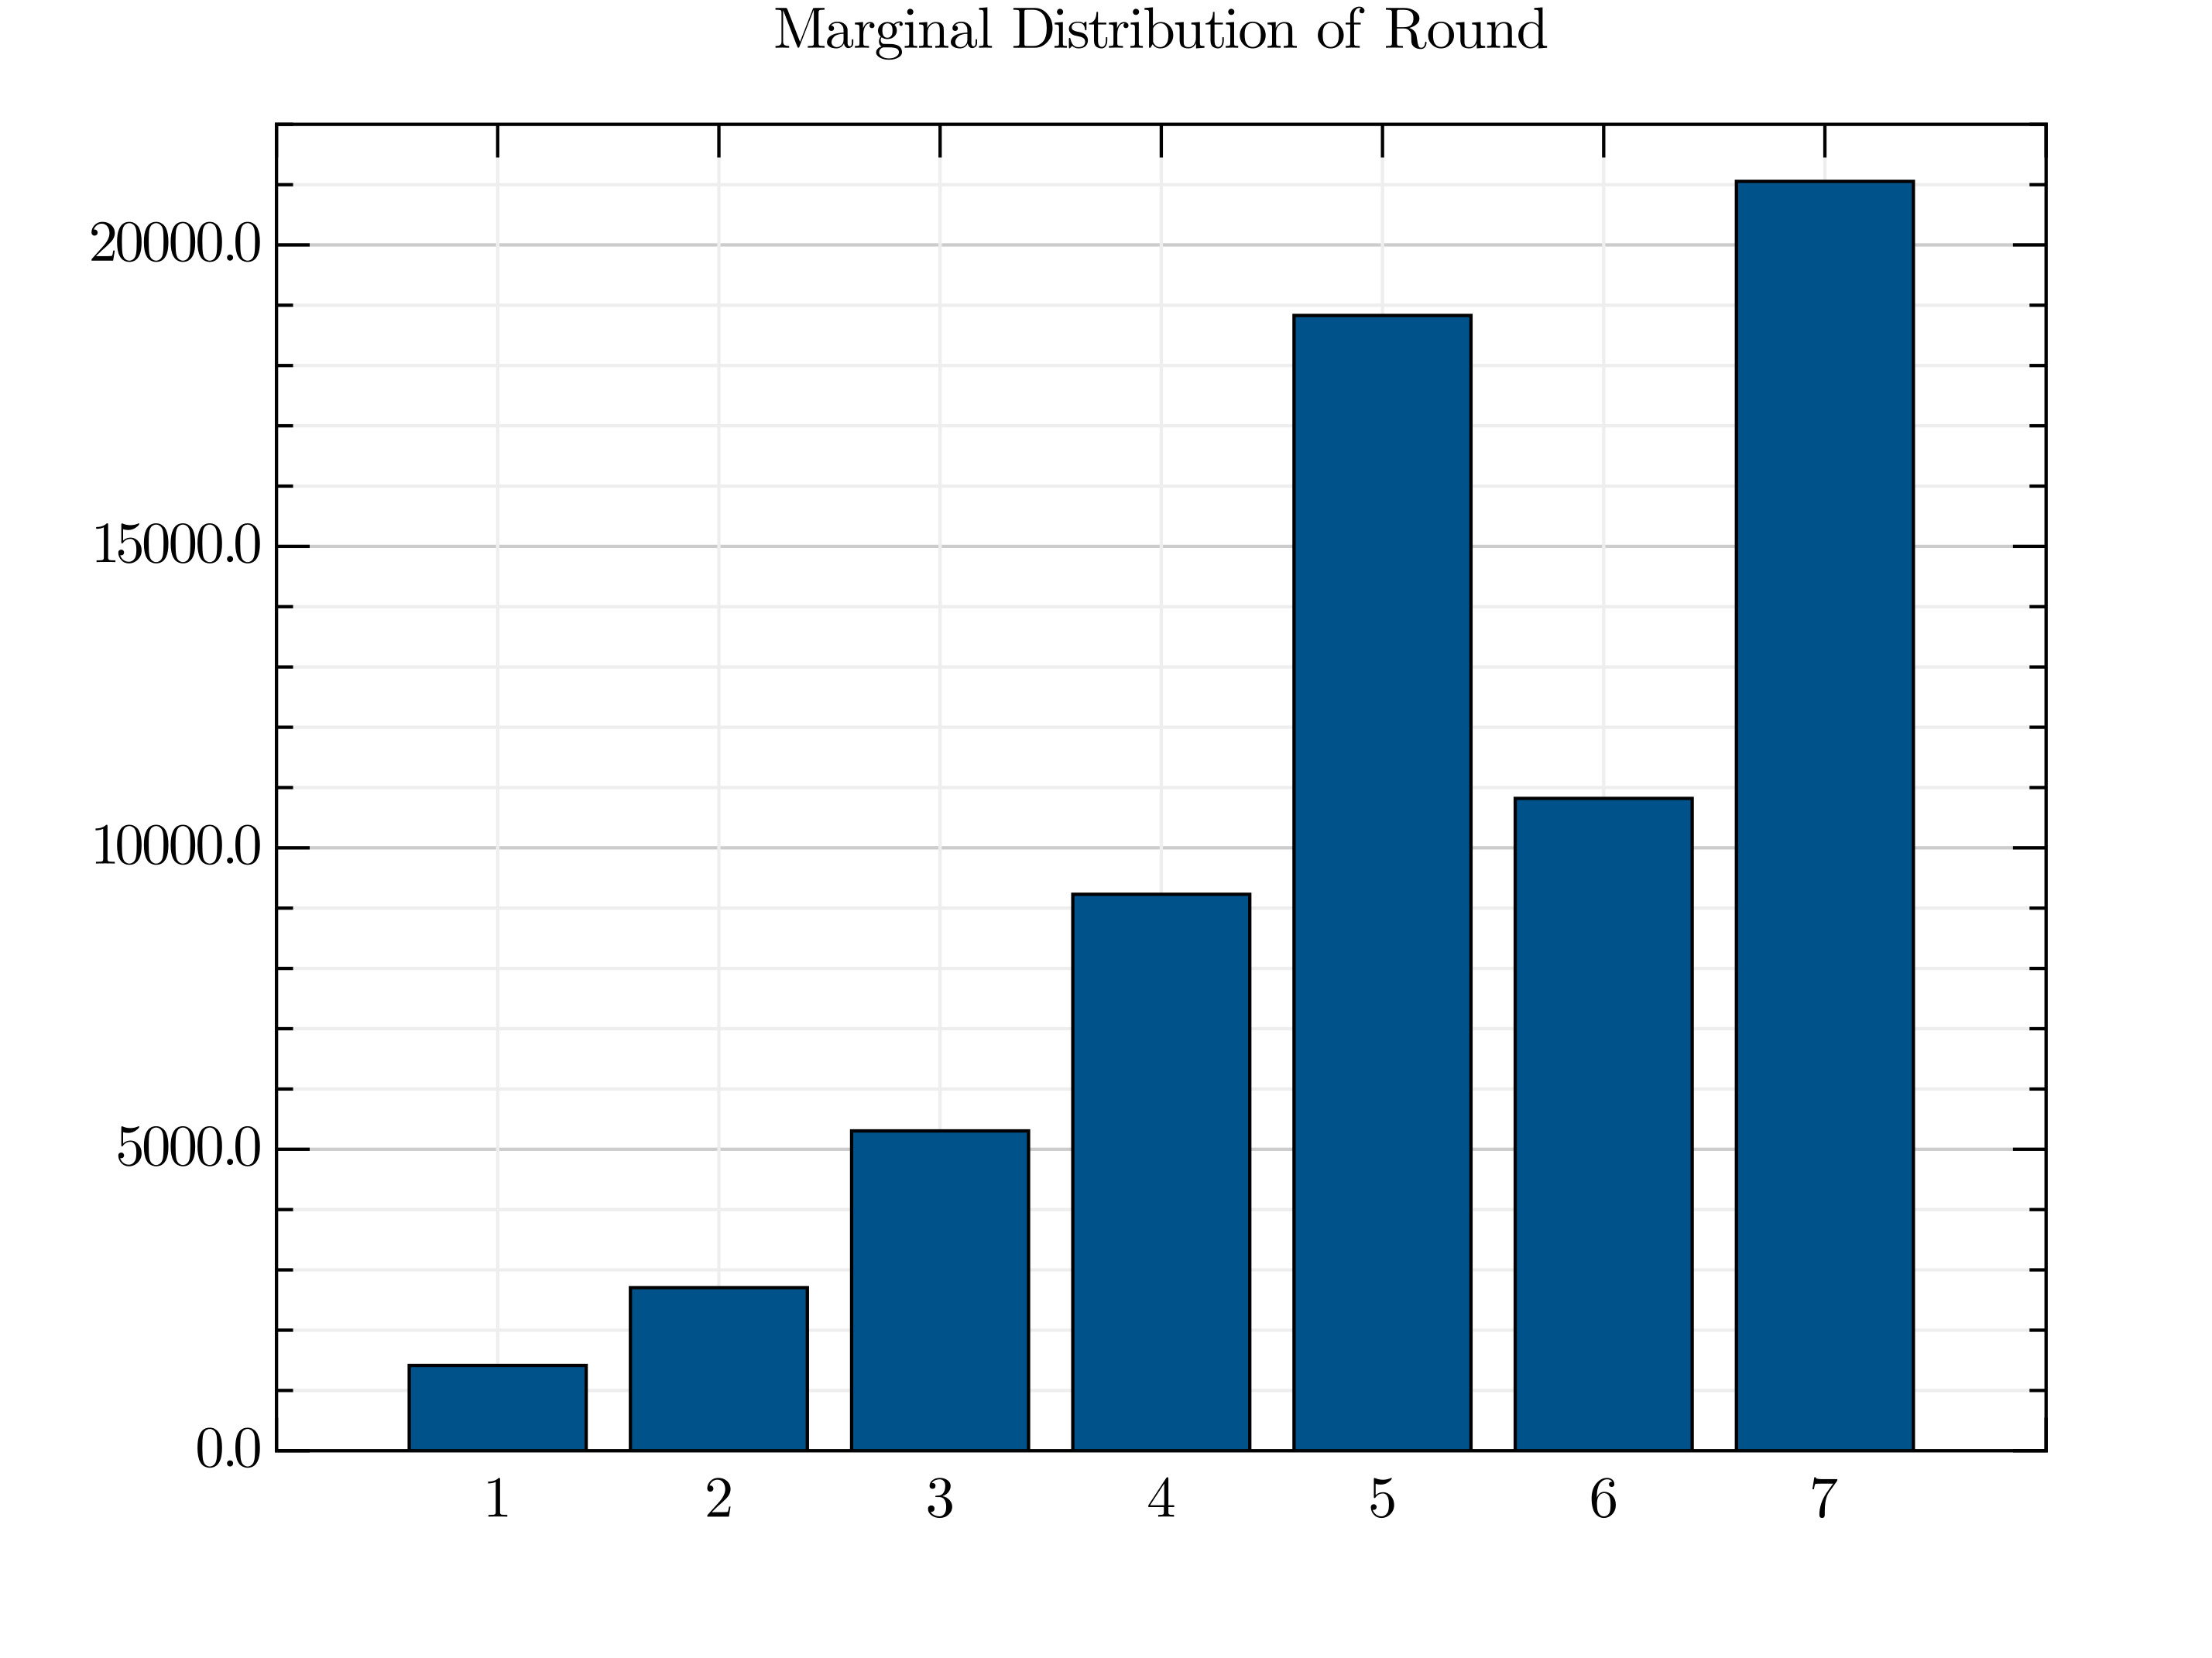
\includegraphics{visuals/marginals_RND.png}
\caption{Judge Origin Marginal}
\end{figure}
 \begin{figure}
\centering
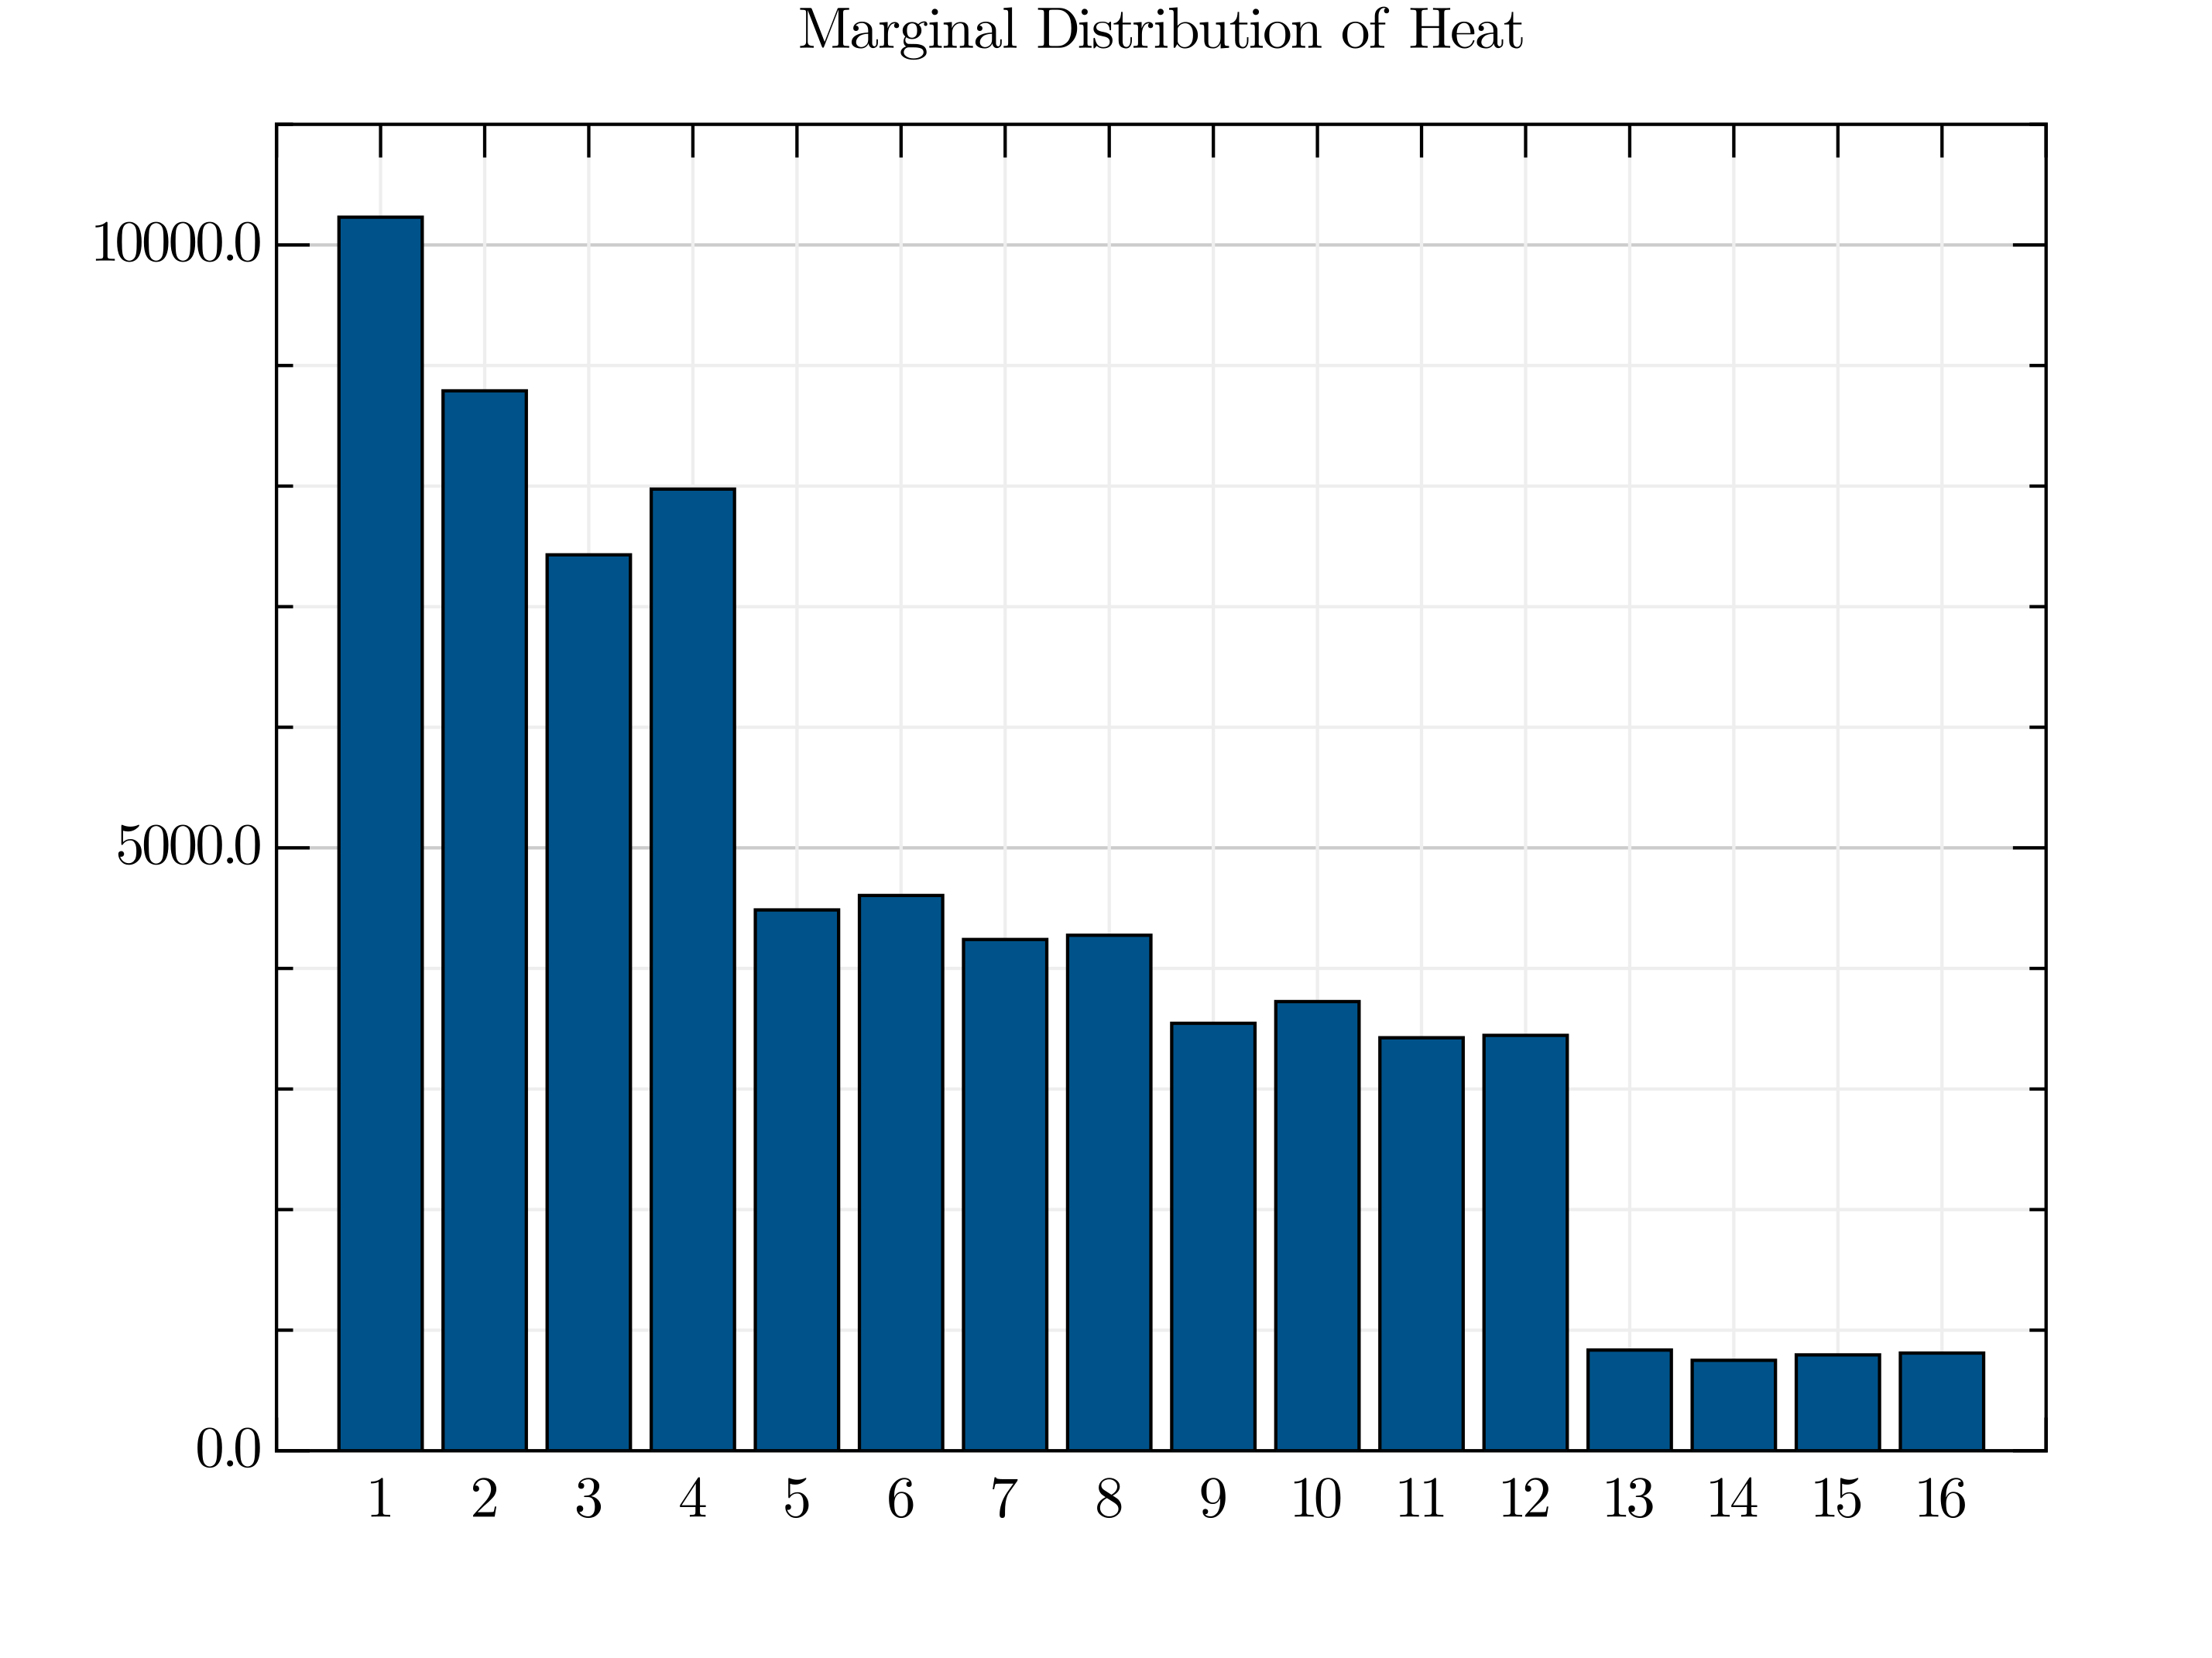
\includegraphics{visuals/marginals_HEAT.png}
\caption{Judge Origin Marginal}
\end{figure}
 \begin{figure}
\centering
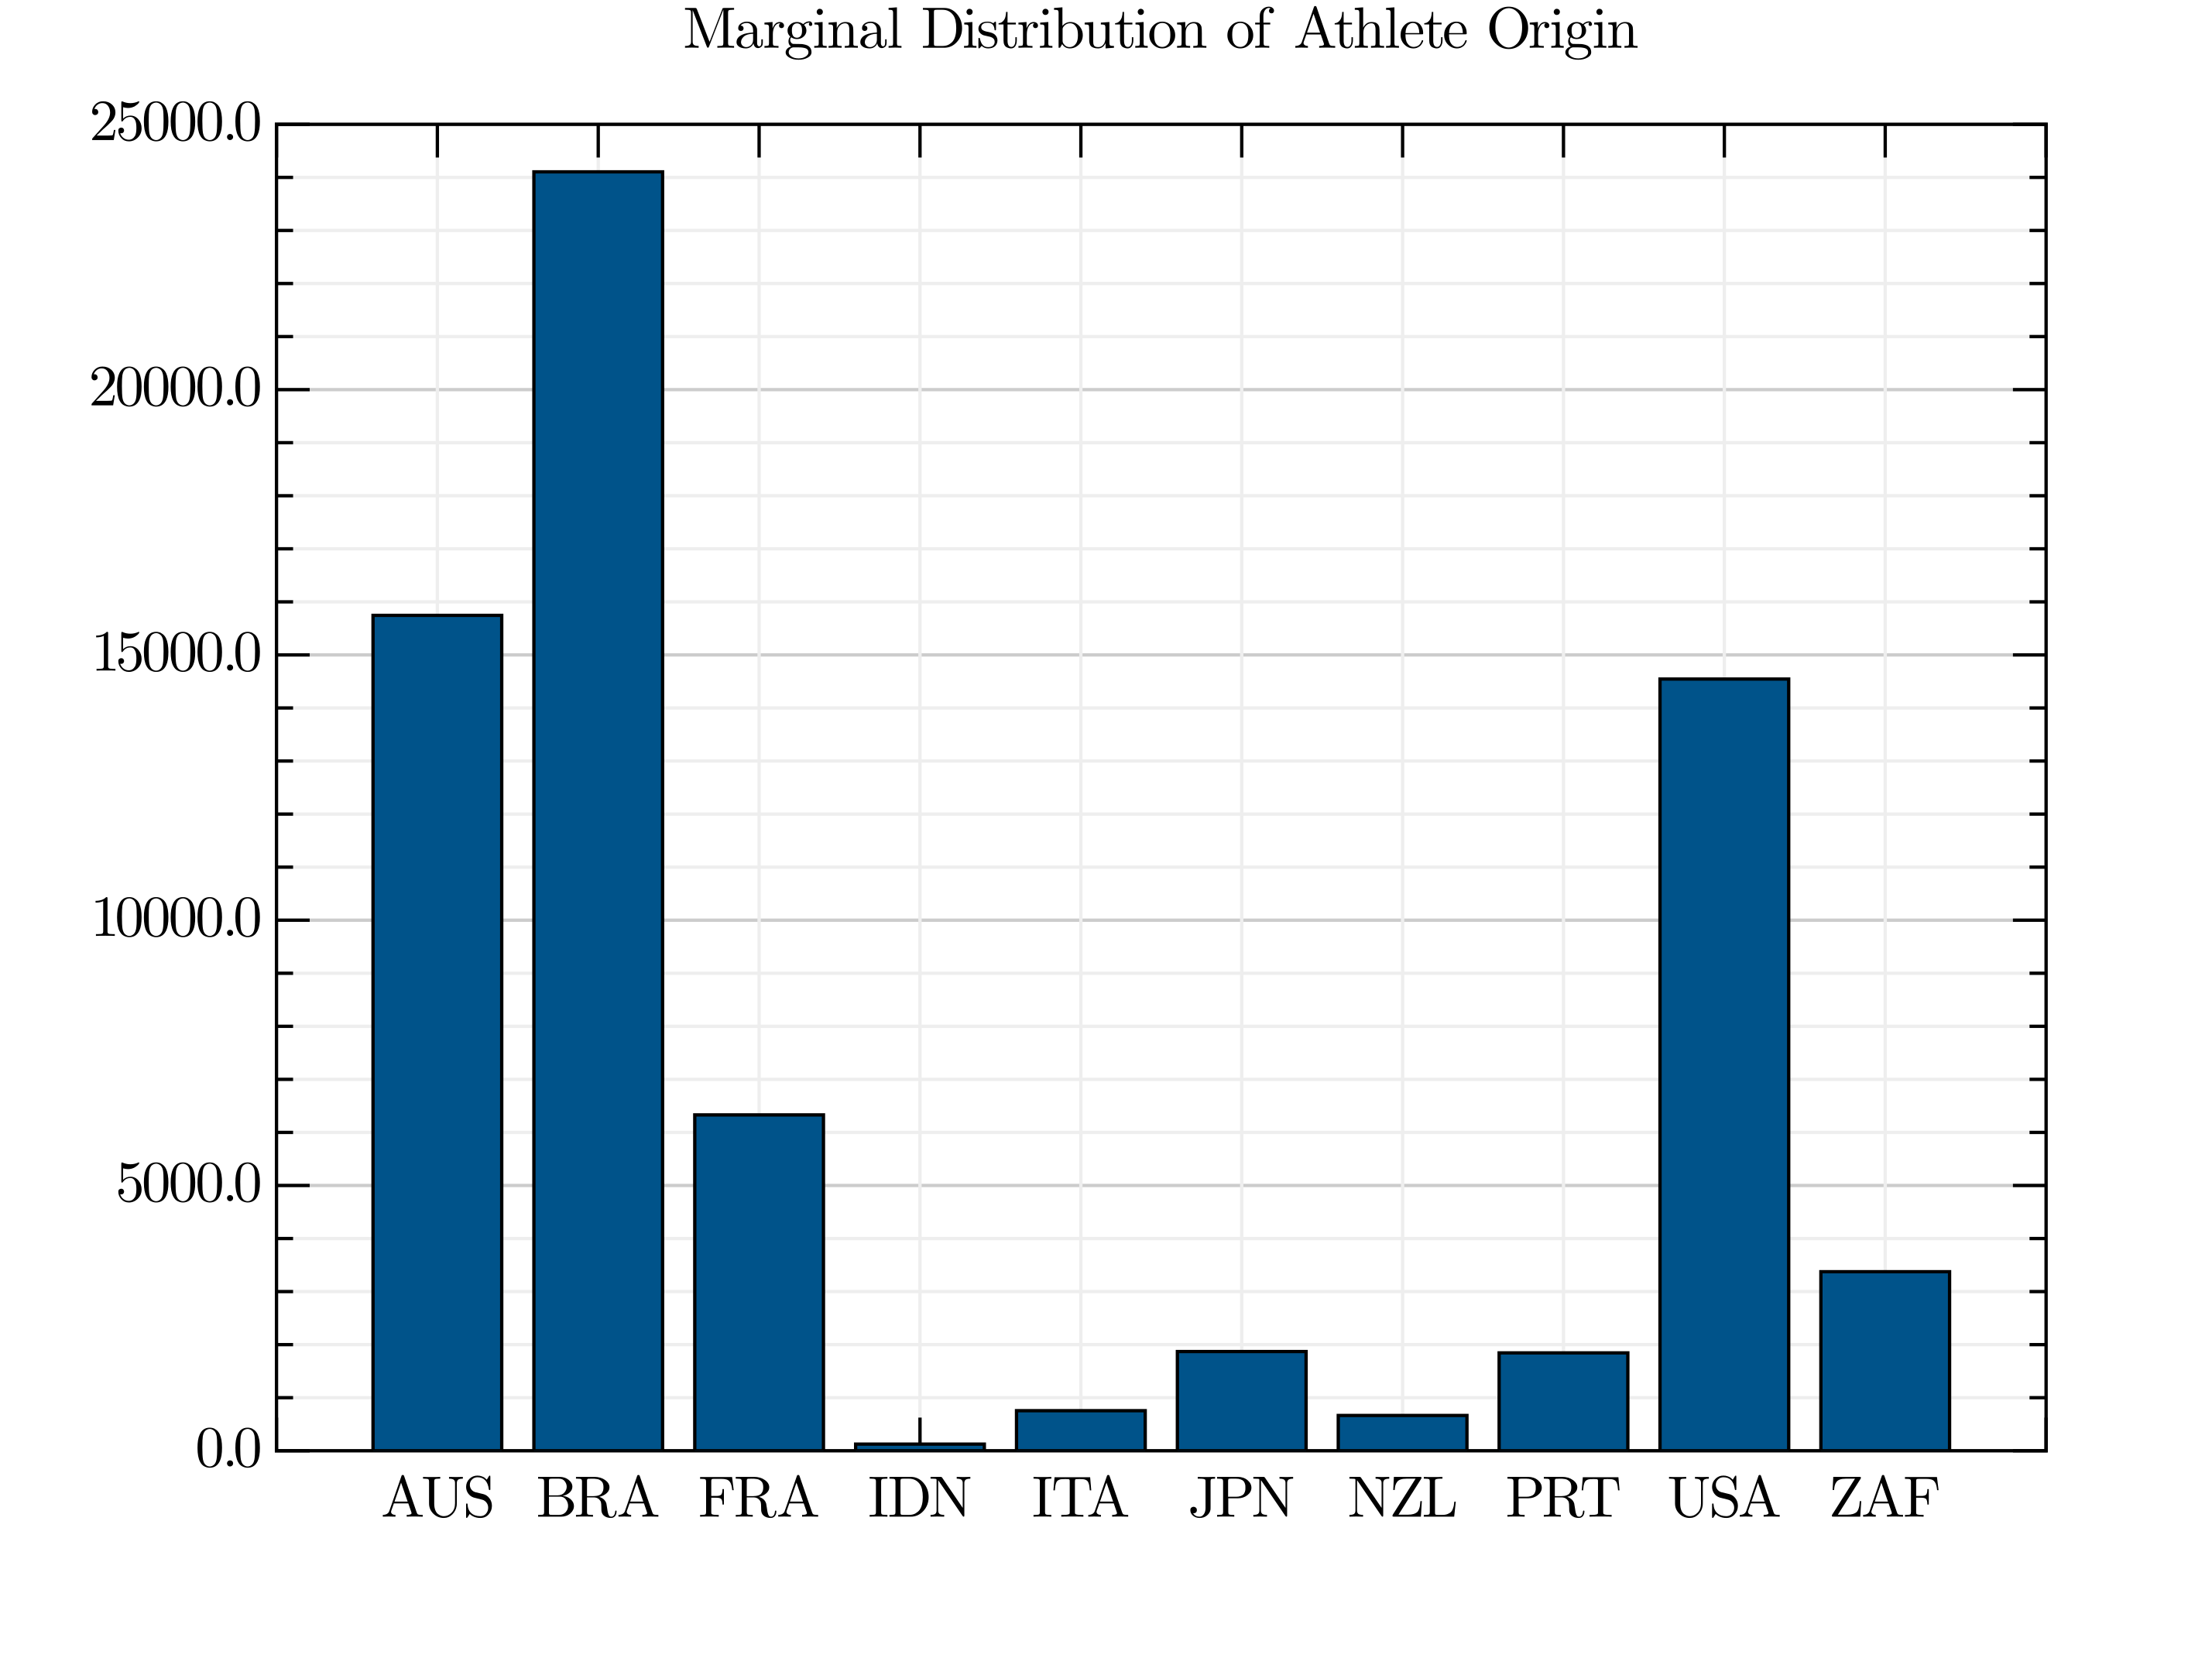
\includegraphics{visuals/marginals_ATH_orig.png}
\caption{Judge Origin Marginal}
\end{figure}
 \begin{figure}
\centering
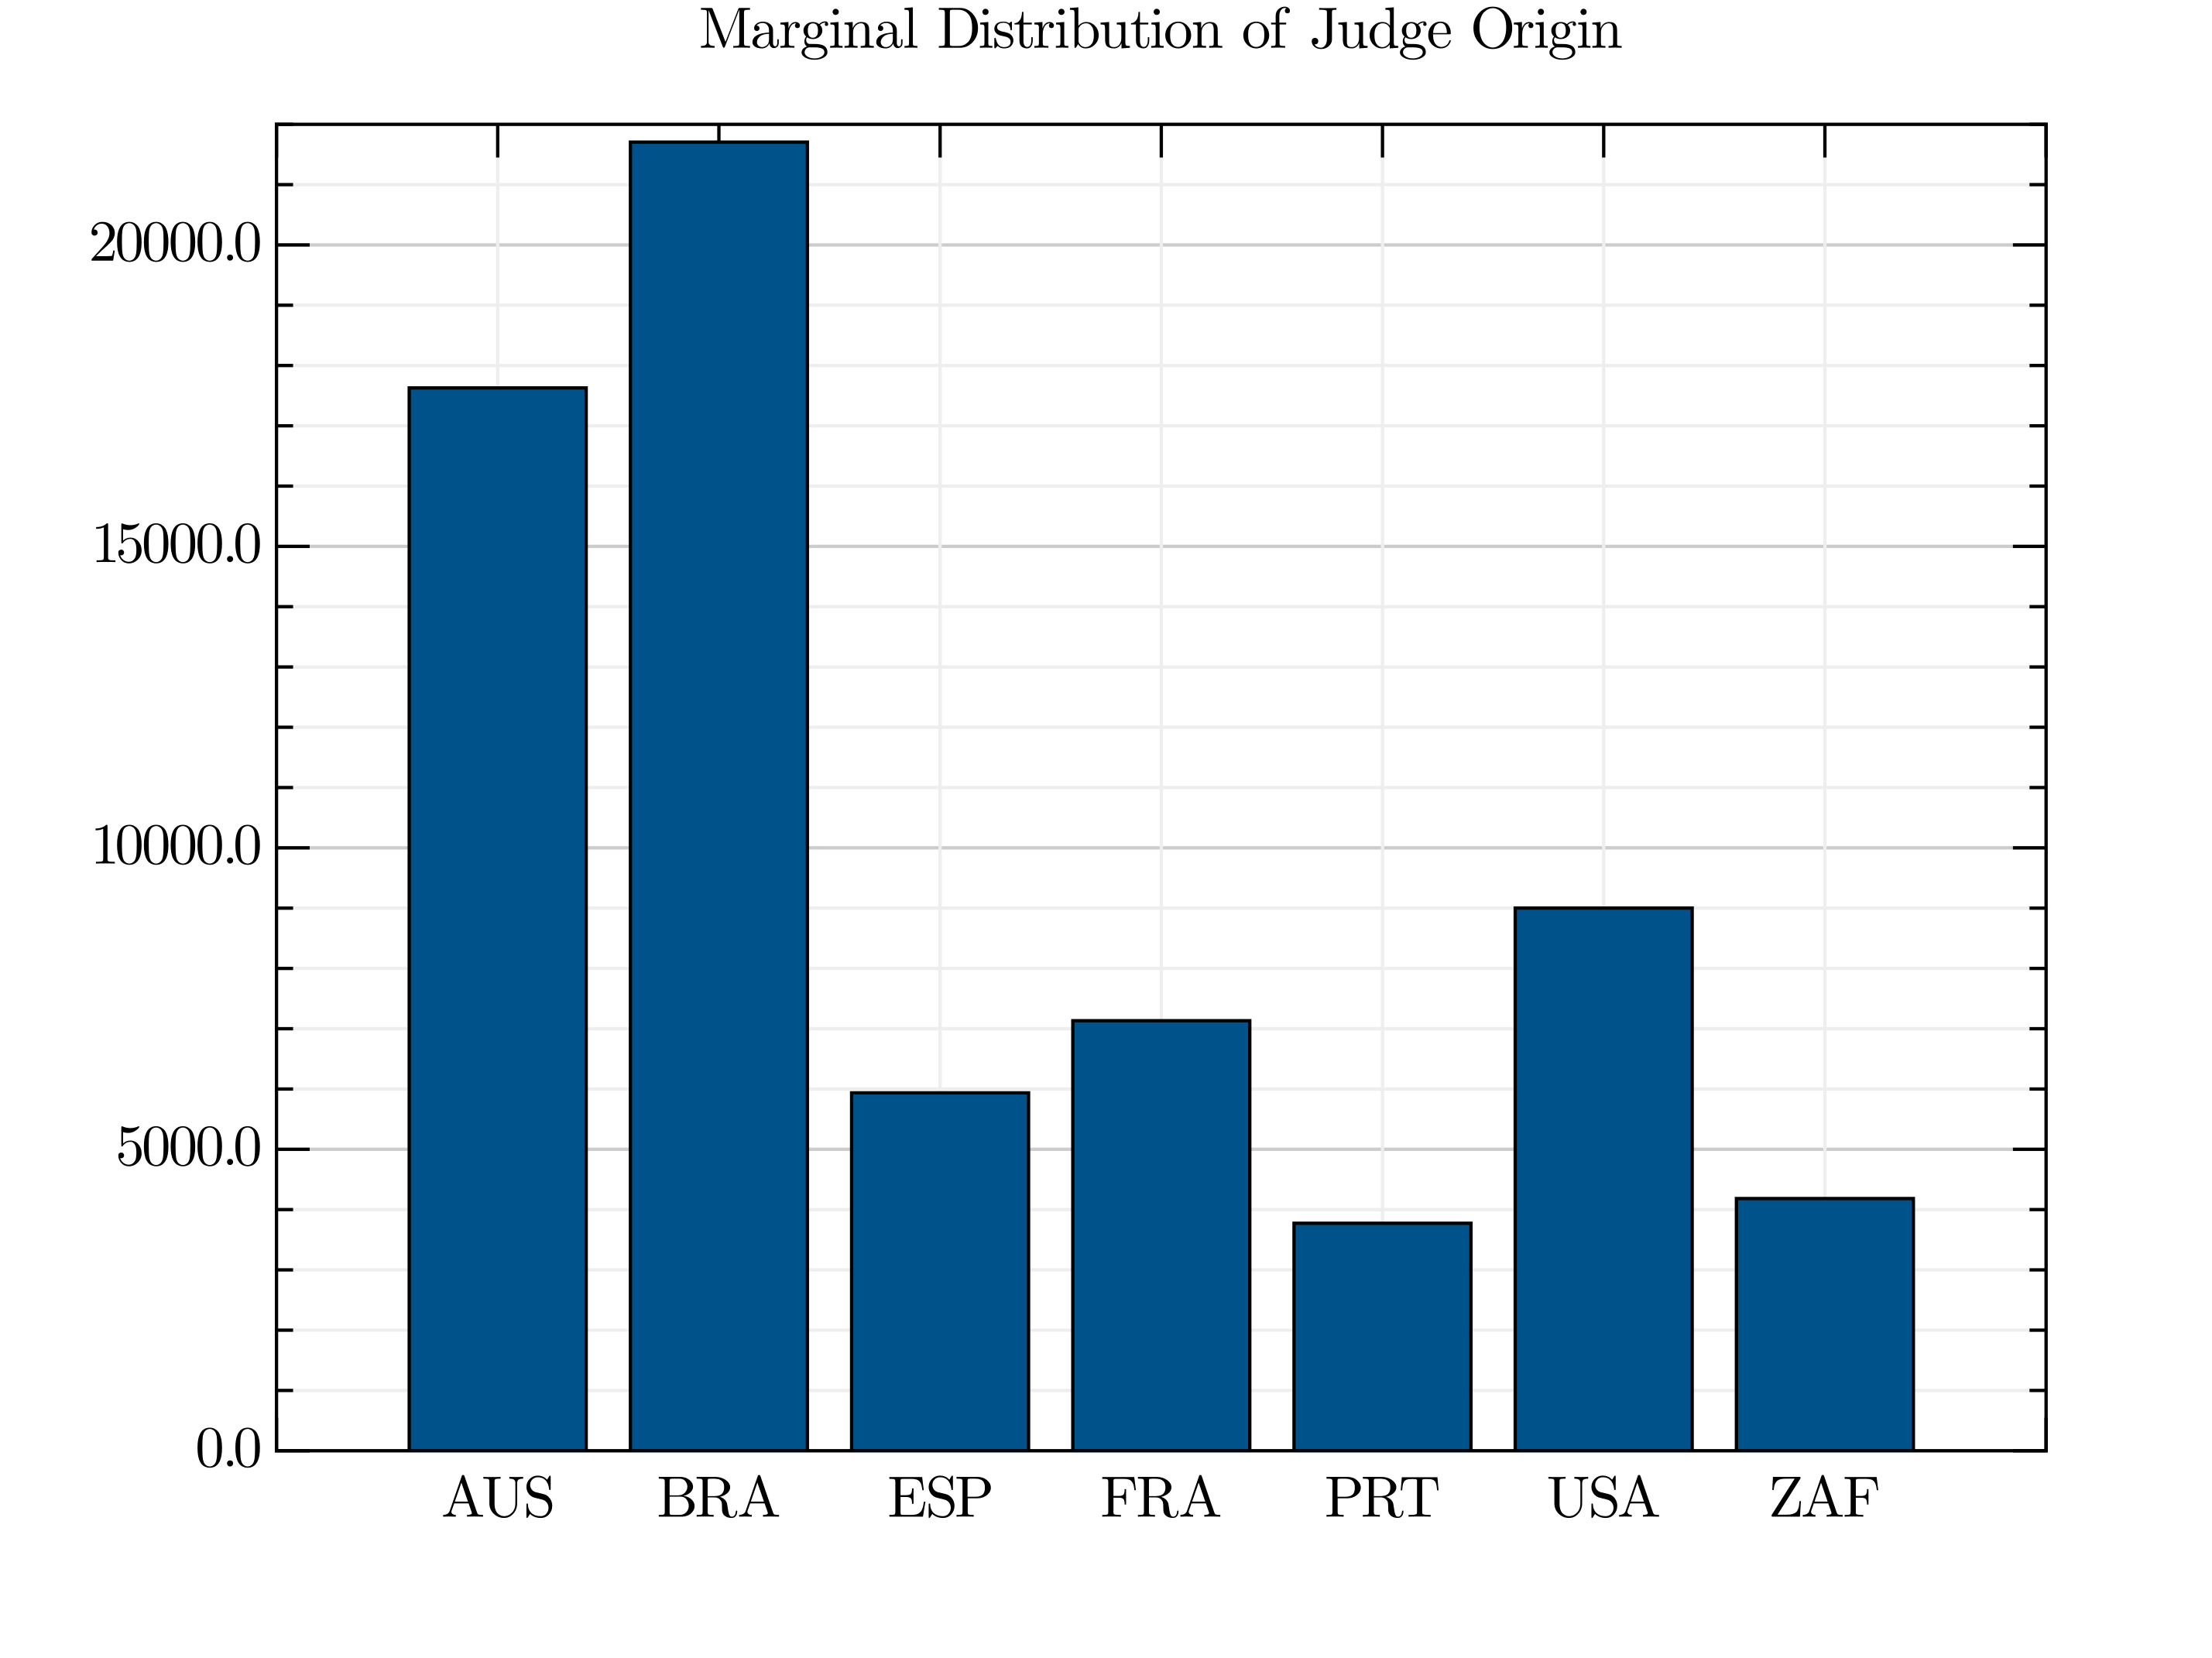
\includegraphics{visuals/marginals_JUD_orig.png}
\caption{Judge Origin Marginal}
\end{figure}
 \begin{figure}
\centering
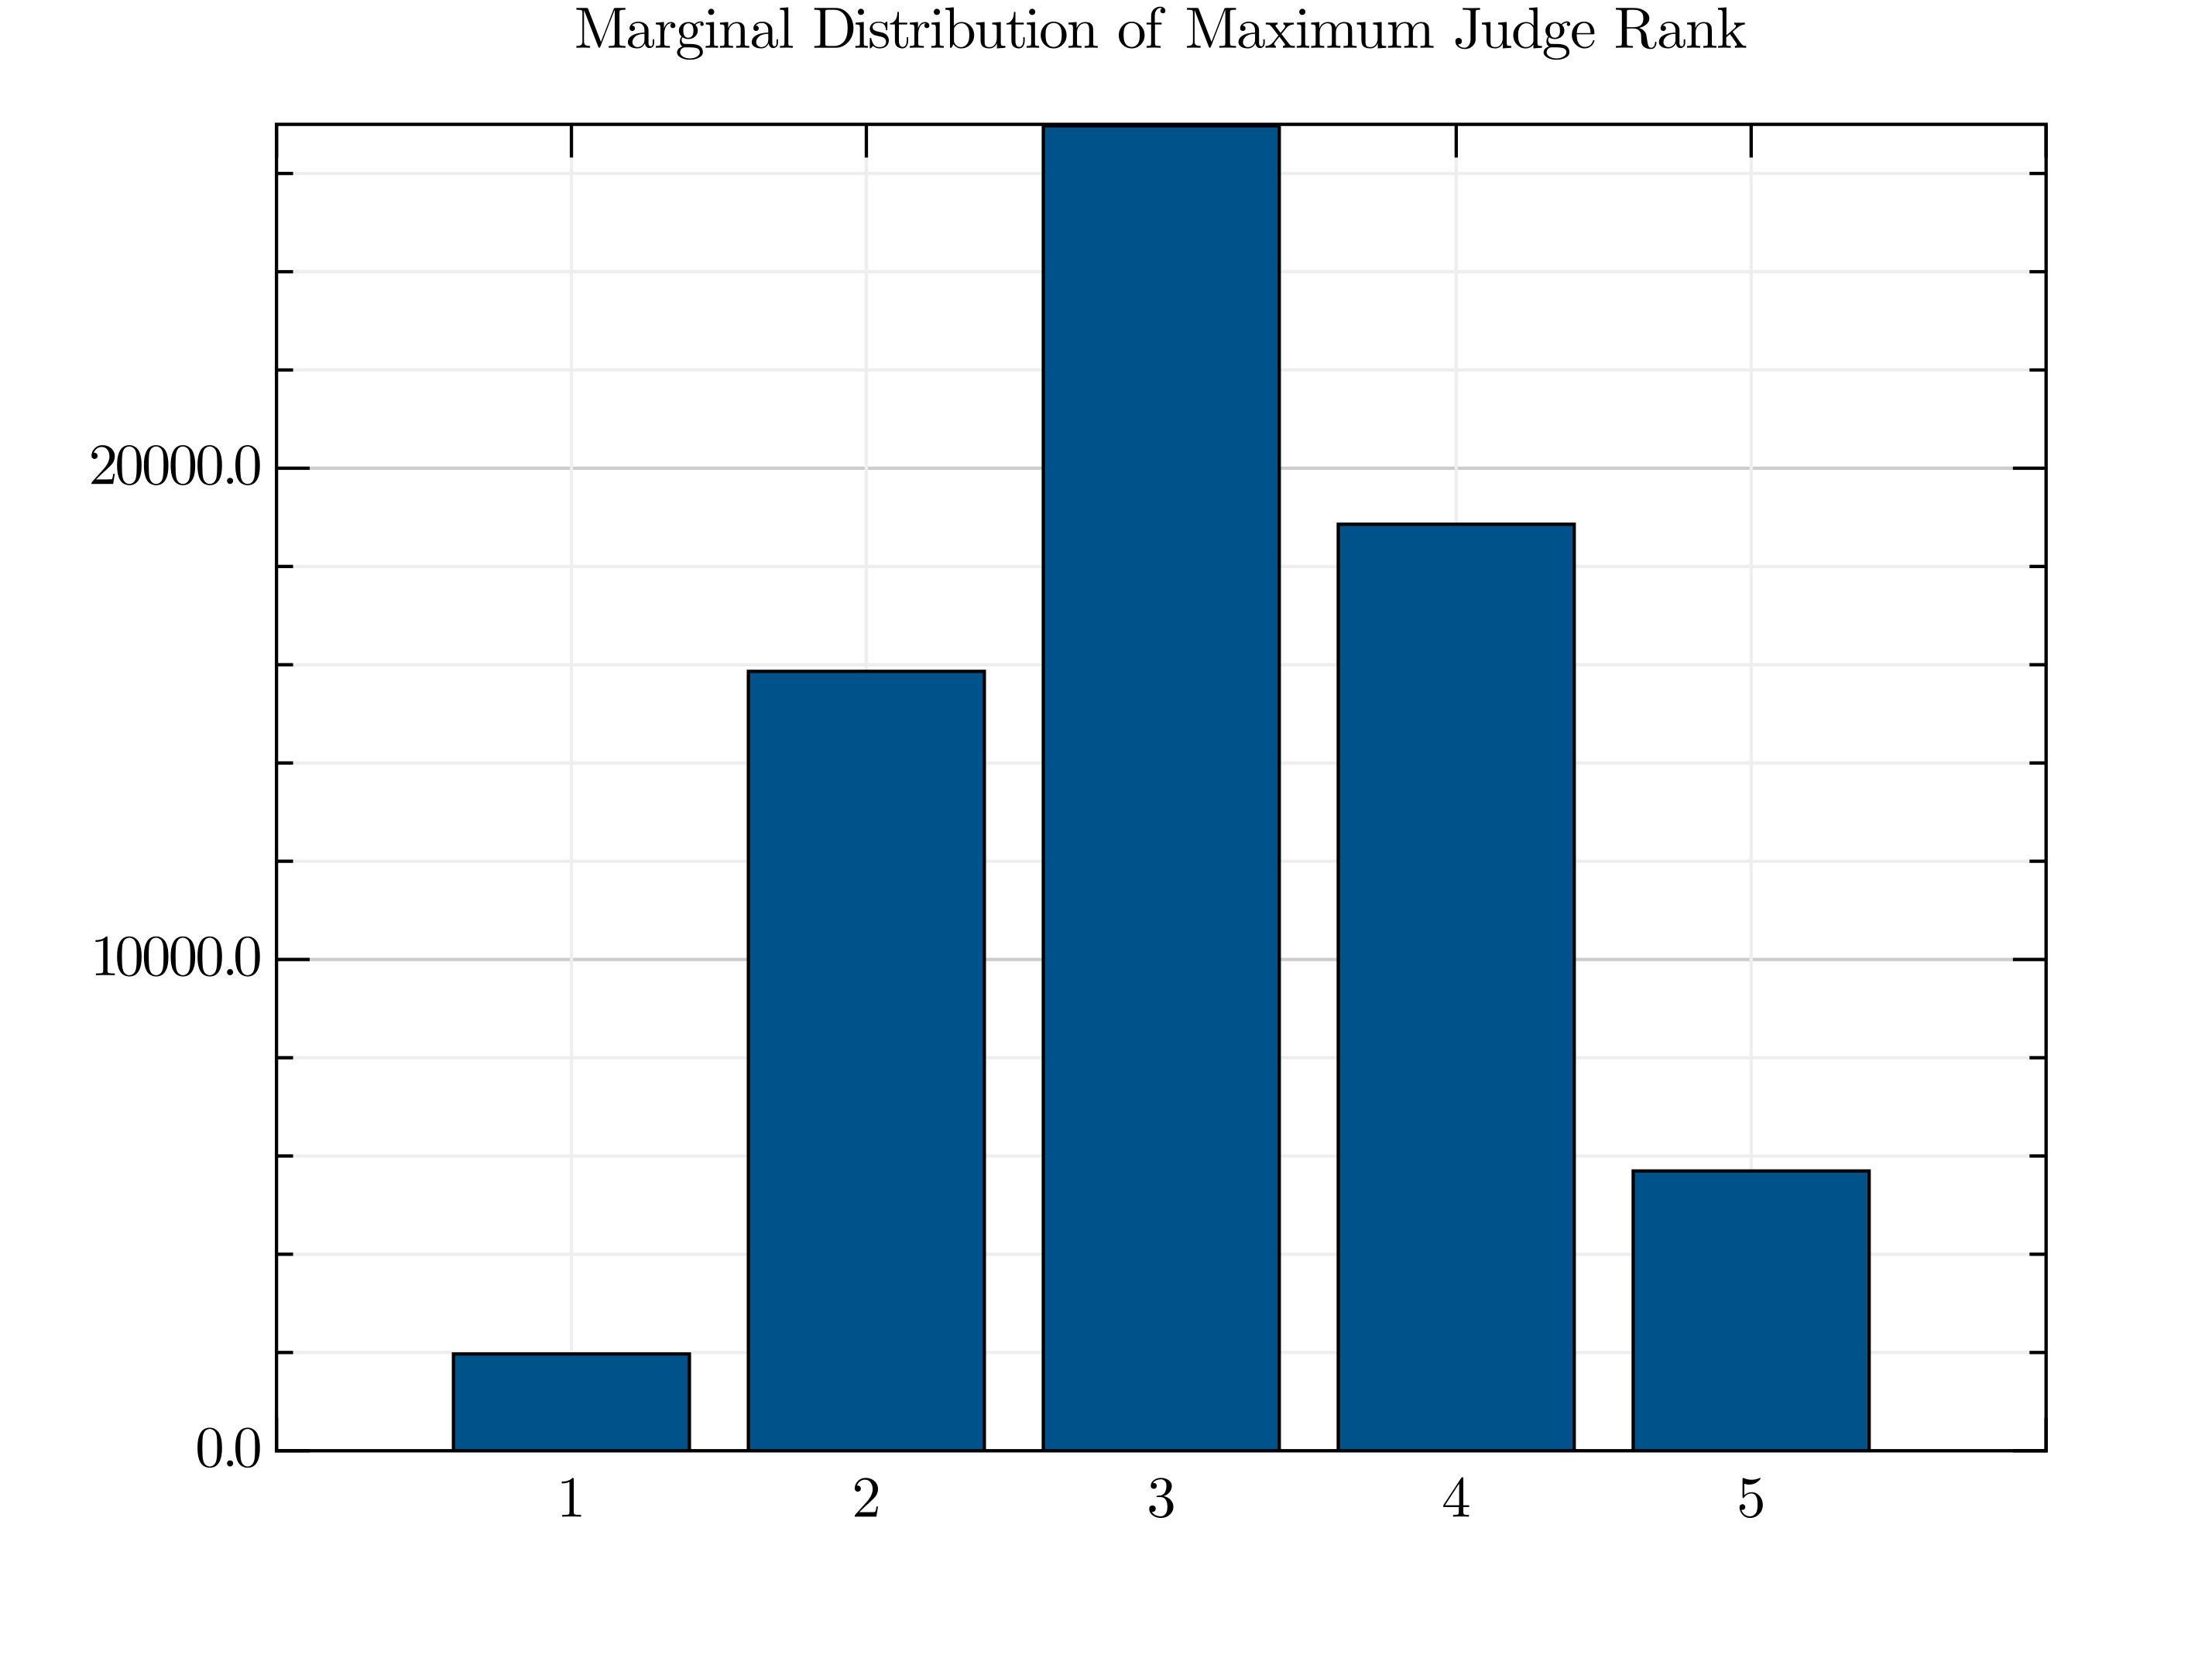
\includegraphics{visuals/marginals_MAX_RANK.png}
\caption{Judge Origin Marginal}
\end{figure}
 \begin{figure}
\centering
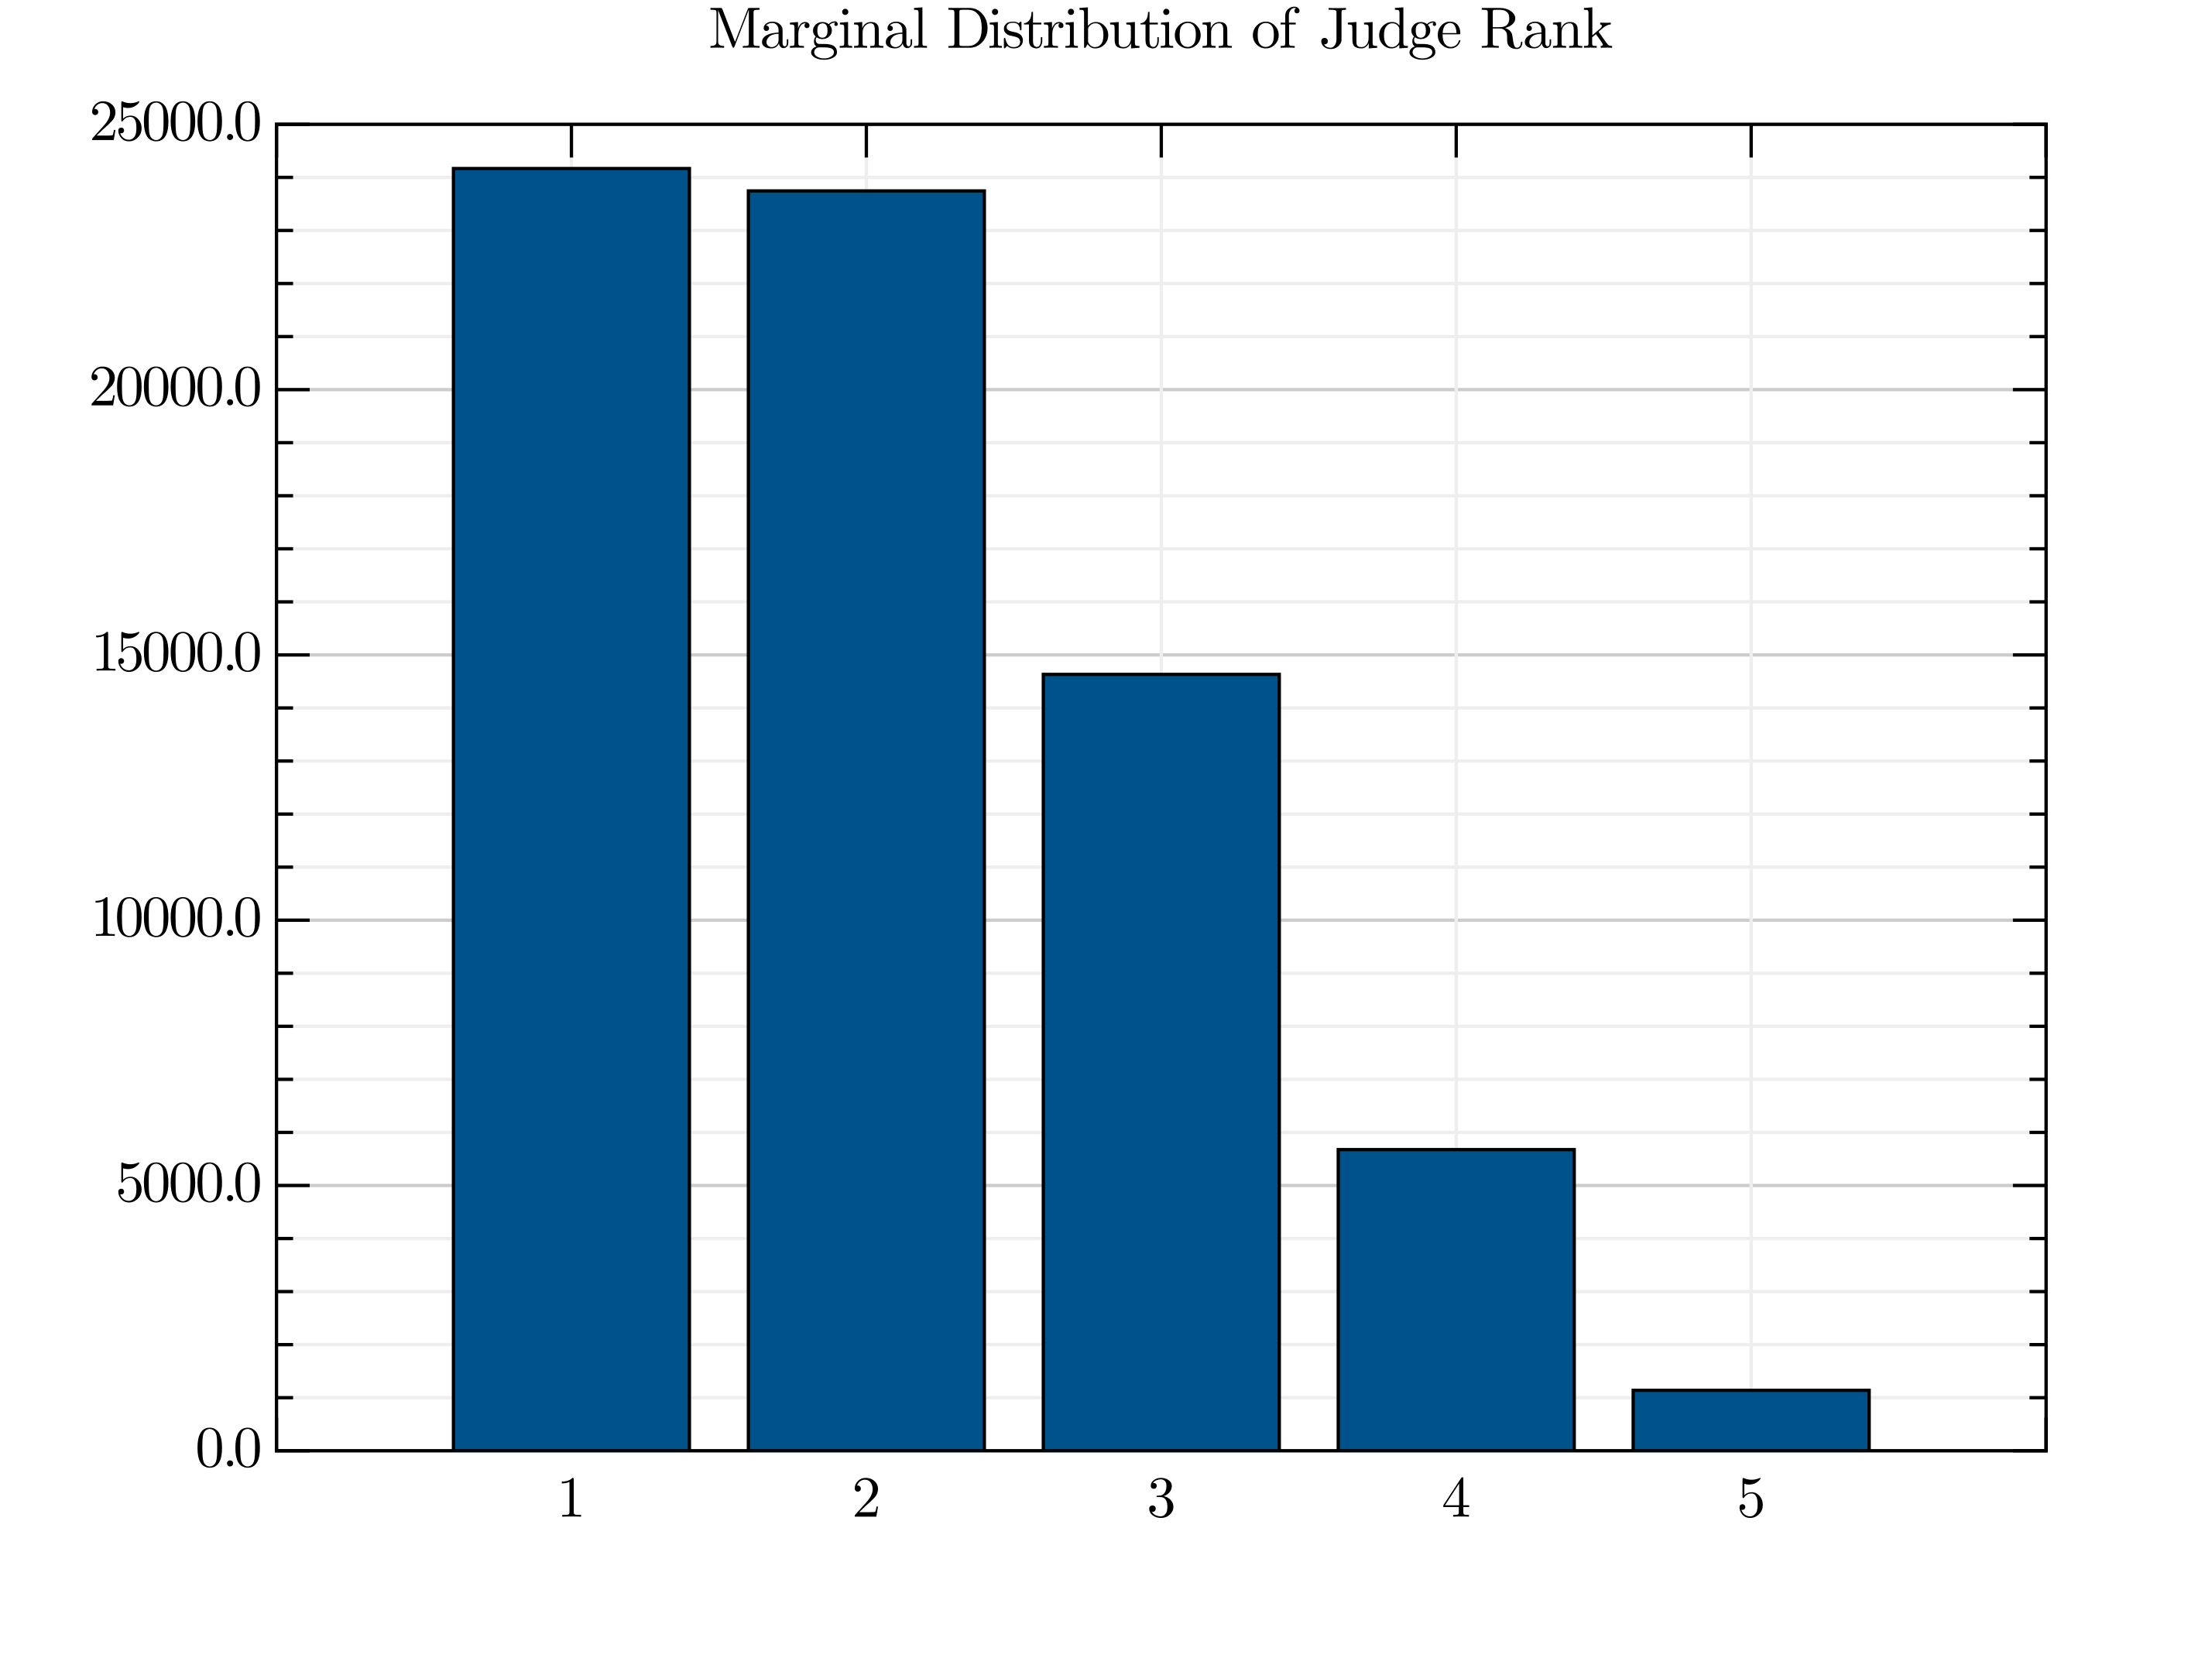
\includegraphics{visuals/marginals_RANK.png}
\caption{Judge Rank Marginal}
\end{figure}



\section{Definitions}
\begin{itemize}
\item \textbf{The Symmetric Group on a set, $X$} is $S_X := Isomorphisms(X,X)$. When $|X|<\infty$,$S_X = \{ \tau :X\rightarrow X \mid Image(\tau) = X \}  = \{\tau:X\rightarrow X \mid \{\tau(x) \mid x \in X\} = X \}$


\item $S_d := S_{\{ 1 ,\dots, d\}}.$


\item When G is a Group, and $\mathbb{F}$ is a Field, the \textbf{Group Algebra of G over $F$}, denoted $\mathbb{F}[G]$, is the space of formal linear combinations of elements of G. Elements of $\mathbb{F}[G]$ are of the form: $c_1 g_1 + \dots + c_n g_n = \sum^n_{i=1} c_i g_i$, where $c_i \in \mathbb{F}, g_i \in G$. Note that $i\neq j \implies g_i \neq g_j$ because G is a set of elements, so no element occurs with multiplicity. For example, $c_1 g + c_2 g \not\in \mathbb{F}[G]$ whereas $(c_1 + c_2)g \in \mathbb{F}[G]$.


\item $\mathbb{F}[S_d]$ is comprised on formal linear combinations of elements of $S_d$. This may be understood as two different ways:

\begin{itemize}
\item There exists a function $a:S_n \rightarrow \mathbb{F}$ and $A :=  \sum_{\tau \in S_d} a(\tau) \tau \quad \in \mathbb{F}[S_n]$.


\item Or: $A = [ \pi_1 \dots  \pi_{d!} ] \begin{bmatrix}a_{\pi_1} \\ \vdots  \\ a_{\pi_{d!}} \end{bmatrix} = \sum_{\tau \in S_d } a_\tau \tau \in \mathbb{F} [S_d]$,where $\tau \in S_d, a_\tau \in \mathbb{F}$.

\end{itemize}

\item \textbf{Addition in $\mathbb{F}[S_n]$} is defined by $A+B = (\sum_{\tau} a_\tau \tau) + (\sum_\tau b_\tau \tau) := \sum_\tau (a_\tau + b_\tau) \tau$


\item \textbf{Scalar Multiplication in $\mathbb{F}[S_d]$} is $c(A) = c(\sum_{\tau} a_\tau \tau)  = \sum_{\tau} ca_\tau \tau$.


\item Multiplication in $\mathbb{F}[S_d]$ is \emph{defined} by: $A*B =(\sum_{\tau} a_\tau \tau)* (\sum_\pi b_\pi \pi) :=\sum_{\gamma \in S_d}(\sum_{\tau,\pi | \tau\pi=\gamma} a_\tau b_\pi) \gamma = \sum_{\gamma \in S_d}(\sum_{  \tau \in S_d} a_\tau b_{\tau^{-1}\gamma} ) \gamma$.

\end{itemize}

We should not over complicate $*$. The \emph{definition} of $*$ may look odd, but it exactly the same as our basic understanding of multiplication: $(\sum_{  \tau} a_\tau\tau) *(\sum_{\pi }   b_\pi \pi) = \sum_{  \tau} (a_\tau\tau) *(\sum_{\pi }   b_\pi \pi) = \sum_{  \tau} \sum_{\pi }  (a_\tau\tau) * (b_\pi \pi) = \sum_{  \tau}\sum_{\pi } a_\tau b_\pi \tau \pi =\sum_{\gamma \in S_d}(\sum_{  \tau,\pi | \tau\pi = \gamma  } a_\tau b_\pi) \gamma =(\sum_{\tau} a_\tau \tau)* (\sum_\pi b_\pi \pi)$ Even though $(\ensuremath{\sum}_{\ensuremath{\tau}} a_\ensuremath{\tau} \ensuremath{\tau}) *(\ensuremath{\sum}_{\ensuremath{\pi}} b_\ensuremath{\pi} \ensuremath{\pi})$ is equal to the intuitive form, $\ensuremath{\sum}_{\ensuremath{\tau}}\sum_{\ensuremath{\pi}} a_\ensuremath{\tau} b_\ensuremath{\pi} \ensuremath{\tau}\ensuremath{\pi}$, the latter is not an element of the the group algebra because elements are repeated in the sum, hence our chosen definition. Also, $*$ merely extends multiplication in the Field,$\cdot: \mathbb{F} \times \mathbb{F} \rightarrow \mathbb{F}$, and the operation in the group, $\ensuremath{\circ}$, by $a_\ensuremath{\tau} \ensuremath{\tau} * b_\ensuremath{\pi} \ensuremath{\pi} = a_\ensuremath{\tau}\ensuremath{\cdot}b_\ensuremath{\pi} \ensuremath{\tau}\ensuremath{\circ}\ensuremath{\pi} = a_\ensuremath{\tau} b_\ensuremath{\pi} \ensuremath{\tau}\ensuremath{\pi}$, where the last equality is simply notation-reduction.

A measure on $S_d$, is an element of the group algebra $\mathbb{C}[S_n]$. A measure on $S_d$, $F = \ensuremath{\sum}_{\ensuremath{\tau} \ensuremath{\in} S_d} f_\ensuremath{\tau} \ensuremath{\tau}$, is a probability measure on $S_d$ if and only if $\ensuremath{\forall} \ensuremath{\tau} \ensuremath{\in} S_d f_\ensuremath{\tau} \geq 0$ and $\ensuremath{\sum}_{\ensuremath{\tau} \ensuremath{\in} S_d} f_\ensuremath{\tau} = 1$.

A linear representation of a group G, is a group homomorphism, $\rho : (G,\circ) \rightarrow (GL(V),\cdot)$. A group homomorphism satisfies:

\begin{itemize}
\item $\ensuremath{\forall} x,y \ensuremath{\in} G \quad \ensuremath{\rho}(x\ensuremath{\circ}y) = \ensuremath{\rho}(x) \cdot \ensuremath{\rho}(y)$ where $\cdot$ is multiplication in $GL(V)$.


\item $\ensuremath{\rho}(e) = I$, where e is the identity element in $G$ and I is the identity element in $GL(V)$.


\item $\ensuremath{\forall} x \ensuremath{\in} G, \ensuremath{\rho}(x^{-1}) = \ensuremath{\rho}(x)^*$, where $^*$ denotes involution in $GL(V)$.

\end{itemize}
The representation of a measure F, is: $\hat{F} := \ensuremath{\sum}_{\ensuremath{\tau} \ensuremath{\in} S_n} P(\ensuremath{\tau}) \ensuremath{\rho}(\ensuremath{\tau})$. Note: This is sometimes called the Fourier transform at a representation, I avoid that lingo. 

\textbf{Convolution of two functions on $S_d$} is a binary operation $A * B := \ensuremath{\sum}_{\ensuremath{\tau} \ensuremath{\in} S_n} a(\ensuremath{\tau}) b(\ensuremath{\tau}^{-1}g)$.

Note: $\widehat{A*B} = \ensuremath{\sum}_{\ensuremath{\gamma}} (A*B)(\ensuremath{\gamma})\ensuremath{\rho}(\ensuremath{\gamma})  = \ensuremath{\sum}_{\ensuremath{\gamma} } \ensuremath{\sum}_{\ensuremath{\tau}} a(\ensuremath{\gamma} \ensuremath{\tau}^{-1})b(\ensuremath{\tau})\rho(\ensuremath{\gamma} ) = \ensuremath{\sum}_{\ensuremath{\tau}} \ensuremath{\sum}_{\ensuremath{\gamma}\ensuremath{\tau}} a(\ensuremath{\gamma} \ensuremath{\tau} \ensuremath{\tau}^{-1})b(\ensuremath{\tau})\ensuremath{\rho}(\ensuremath{\gamma}\ensuremath{\tau}) = \ensuremath{\sum}_{\ensuremath{\tau}} \ensuremath{\sum}_{\ensuremath{\gamma}\ensuremath{\tau}} a(\ensuremath{\gamma})b(\ensuremath{\tau})\ensuremath{\rho}(\ensuremath{\gamma})\ensuremath{\rho}(\ensuremath{\tau}) = \ensuremath{\sum}_{\ensuremath{\tau}} b(\ensuremath{\tau})\ensuremath{\rho}(\ensuremath{\tau}) \ensuremath{\sum}_{\ensuremath{\gamma}\ensuremath{\tau}} a(\ensuremath{\gamma})\ensuremath{\rho}(\ensuremath{\gamma})  = \ensuremath{\sum}_{\ensuremath{\tau}} b(\ensuremath{\tau})\ensuremath{\rho}(\ensuremath{\tau}) \hat{A} = \hat{A} \ensuremath{\sum}_{\ensuremath{\tau}} b(\ensuremath{\tau})\rho(\ensuremath{\tau}) = \hat{A} \cdot \hat{B}$

We take $\ensuremath{\rho}_d$ the permutation representation acting on the vector space $V := \mathbb{R}^d$ with basis indexed by $\{1,\ensuremath{\ldots},d\}$. So a typical element of V is of the form: 

$\begin{pmatrix} a^1 \\ a^2 \\ \vdots \\ a^n \end{pmatrix} = \begin{pmatrix} a^1 \\ 0 \\ \vdots \\ 0 \end{pmatrix} + \begin{pmatrix} 0 \\ a^2 \\ \vdots \\ 0 \end{pmatrix} + \dots + \begin{pmatrix} 0 \\  \vdots \\ 0\\ a^n \end{pmatrix}  = a^1\begin{pmatrix} 1 \\ 0 \\ \vdots \\ 0 \end{pmatrix} + a^2\begin{pmatrix} 0 \\ 1 \\ \vdots \\ 0 \end{pmatrix} + \dots + a^n\begin{pmatrix} 0 \\  \vdots \\ 0\\ 1\end{pmatrix}  = a^1 e_1 + a^2 e_2 + \dots a^n e_n$

This could be rewritten as $\ensuremath{\sum}_{i \ensuremath{\in} \{1,\ensuremath{\ldots},n\} } a^i e_i$. But remember, we are interested in functions that act on the basis.

Many authors call $*$ "convolution", however this terminology is superfluous.

\section{Analysis}
One thing I could change:

\begin{itemize}
\item instead giving every element of rth partition rank  give them each:

\end{itemize}
\{ N\ensuremath{\_r} + i for i in 1:n\_i\}  where N\ensuremath{\_r} is \ensuremath{\Sigma}\ensuremath{\^r}n\ensuremath{\_i} ... but then any answer we give loses meaning

I wonder: M\ensuremath{\_r} := max order for that wave B = 1\emph{\{order(J\ensuremath{\_i}) = 1 \} T = 1}\{order(J\ensuremath{\_i}) = M\ensuremath{\_r} \} B \ensuremath{\cup} T only really meaninful for M\ensuremath{\_r}>2

Wondering\ensuremath{\_1}: if P(T | JUD\emph{orig==ATH}orig ) =  P( T | JUD\emph{orig != ATH}orig ) Wondering\ensuremath{\_2}: if Wondering\ensuremath{\_1} depends on [   ]\emph{orig Wondering\ensuremath{\_3}: if P( B \ensuremath{\cup} T | M\ensuremath{\_r} ) = 2/M\ensuremath{\_r} Wondering\ensuremath{\_4}: if P(T | (JUD}orig==ATH\_orig,M\ensuremath{\_r}) ) = 1/M\ensuremath{\_r}


\subsection{Method 1}

\begin{lstlisting}
(*@\HLJLn{ATHandJUD{\_}orig}@*) (*@\HLJLoB{=}@*) (*@\HLJLnf{intersect}@*)(*@\HLJLp{(}@*)(*@\HLJLnf{keys}@*)(*@\HLJLp{(}@*)(*@\HLJLn{ToInd}@*)(*@\HLJLp{[}@*)(*@\HLJLsc{:ATH{\_}orig}@*)(*@\HLJLp{]),}@*)(*@\HLJLnf{keys}@*)(*@\HLJLp{(}@*)(*@\HLJLn{ToInd}@*)(*@\HLJLp{[}@*)(*@\HLJLsc{:JUD{\_}orig}@*)(*@\HLJLp{])}@*) (*@\HLJLp{)}@*)

(*@\HLJLn{GivenMatchByM\ensuremath{\_r}}@*) (*@\HLJLoB{=}@*) (*@\HLJLp{[}@*)
(*@\HLJLnf{sum}@*)(*@\HLJLp{(}@*) (*@\HLJLp{[}@*) (*@\HLJLnf{sum}@*)(*@\HLJLp{(}@*)(*@\HLJLn{info}@*)(*@\HLJLp{[}@*)(*@\HLJLoB{:}@*)(*@\HLJLp{,}@*)(*@\HLJLoB{:}@*)(*@\HLJLp{,}@*)(*@\HLJLoB{:}@*)(*@\HLJLp{,}@*)(*@\HLJLoB{:}@*)(*@\HLJLp{,}@*)(*@\HLJLn{ToInd}@*)(*@\HLJLp{[}@*)(*@\HLJLsc{:ATH{\_}orig}@*)(*@\HLJLp{][}@*)(*@\HLJLn{c}@*)(*@\HLJLp{],}@*)(*@\HLJLn{ToInd}@*)(*@\HLJLp{[}@*)(*@\HLJLsc{:JUD{\_}orig}@*)(*@\HLJLp{][}@*)(*@\HLJLn{c}@*)(*@\HLJLp{],}@*)(*@\HLJLn{r}@*)(*@\HLJLp{,}@*)(*@\HLJLoB{:}@*)(*@\HLJLp{])}@*) (*@\HLJLk{for}@*) (*@\HLJLn{c}@*) (*@\HLJLkp{in}@*) (*@\HLJLn{ATHandJUD{\_}orig}@*) (*@\HLJLp{]}@*) (*@\HLJLp{)}@*)
(*@\HLJLk{for}@*) (*@\HLJLn{r}@*) (*@\HLJLkp{in}@*) (*@\HLJLni{1}@*)(*@\HLJLoB{:}@*)(*@\HLJLni{5}@*)
(*@\HLJLp{]}@*)
(*@\HLJLnf{println}@*)(*@\HLJLp{(}@*)(*@\HLJLs{"{}Match}@*) (*@\HLJLs{conditional}@*) (*@\HLJLs{on}@*) (*@\HLJLs{Max}@*) (*@\HLJLs{Rank}@*) (*@\HLJLs{is:"{}}@*)(*@\HLJLp{)}@*)
(*@\HLJLn{GivenMatchByM\ensuremath{\_r}}@*)

(*@\HLJLn{TopGivenMatchByM\ensuremath{\_r}}@*) (*@\HLJLoB{=}@*) (*@\HLJLp{[}@*)
(*@\HLJLnf{sum}@*)(*@\HLJLp{(}@*) (*@\HLJLp{[}@*) (*@\HLJLnf{sum}@*)(*@\HLJLp{(}@*)(*@\HLJLn{info}@*)(*@\HLJLp{[}@*)(*@\HLJLoB{:}@*)(*@\HLJLp{,}@*)(*@\HLJLoB{:}@*)(*@\HLJLp{,}@*)(*@\HLJLoB{:}@*)(*@\HLJLp{,}@*)(*@\HLJLoB{:}@*)(*@\HLJLp{,}@*)(*@\HLJLn{ToInd}@*)(*@\HLJLp{[}@*)(*@\HLJLsc{:ATH{\_}orig}@*)(*@\HLJLp{][}@*)(*@\HLJLn{c}@*)(*@\HLJLp{],}@*)(*@\HLJLn{ToInd}@*)(*@\HLJLp{[}@*)(*@\HLJLsc{:JUD{\_}orig}@*)(*@\HLJLp{][}@*)(*@\HLJLn{c}@*)(*@\HLJLp{],}@*)(*@\HLJLn{r}@*)(*@\HLJLp{,}@*)(*@\HLJLni{1}@*)(*@\HLJLp{])}@*) 
(*@\HLJLk{for}@*) (*@\HLJLn{c}@*) (*@\HLJLkp{in}@*) (*@\HLJLn{ATHandJUD{\_}orig}@*)(*@\HLJLp{])}@*)
(*@\HLJLk{for}@*) (*@\HLJLn{r}@*) (*@\HLJLkp{in}@*) (*@\HLJLni{1}@*)(*@\HLJLoB{:}@*)(*@\HLJLni{5}@*)
(*@\HLJLp{]}@*)
(*@\HLJLnf{println}@*)(*@\HLJLp{(}@*)(*@\HLJLs{"{}Judge}@*) (*@\HLJLs{has}@*) (*@\HLJLs{Max}@*) (*@\HLJLs{Rank}@*) (*@\HLJLs{given}@*) (*@\HLJLs{Match}@*) (*@\HLJLs{(by}@*) (*@\HLJLs{Max}@*) (*@\HLJLs{Rank)"{}}@*)(*@\HLJLp{)}@*)
(*@\HLJLn{TopGivenMatchByM\ensuremath{\_r}}@*)

(*@\HLJLn{D\ensuremath{\_1}}@*) (*@\HLJLoB{=}@*) (*@\HLJLn{TopGivenMatchByM\ensuremath{\_r}}@*) (*@\HLJLoB{./}@*) (*@\HLJLn{GivenMatchByM\ensuremath{\_r}}@*)
\end{lstlisting}

\begin{lstlisting}
Match conditional on Max Rank is:
Judge has Max Rank given Match (by Max Rank)
5-element Array(*@{{\{}}@*)Float64,1(*@{{\}}}@*):
 1.0
 0.4969289265867213
 0.3061258835408953
 0.21223286661753868
 0.18444995864350702
\end{lstlisting}


We would expect:


\begin{lstlisting}
(*@\HLJLn{E\ensuremath{\_1}}@*) (*@\HLJLoB{=}@*) (*@\HLJLp{[}@*)(*@\HLJLni{1}@*)(*@\HLJLoB{/}@*)(*@\HLJLn{r}@*) (*@\HLJLk{for}@*) (*@\HLJLn{r}@*) (*@\HLJLkp{in}@*) (*@\HLJLni{1}@*)(*@\HLJLoB{:}@*)(*@\HLJLni{5}@*)(*@\HLJLp{]}@*)
\end{lstlisting}

\begin{lstlisting}
5-element Array(*@{{\{}}@*)Float64,1(*@{{\}}}@*):
 1.0
 0.5
 0.3333333333333333
 0.25
 0.2
\end{lstlisting}


So we have:


\begin{lstlisting}
(*@\HLJLn{\ensuremath{\chi}sq\ensuremath{\_1}}@*) (*@\HLJLoB{=}@*) (*@\HLJLnf{sum}@*)(*@\HLJLp{(}@*)(*@\HLJLn{GivenMatchByM\ensuremath{\_r}}@*)(*@\HLJLp{)}@*)(*@\HLJLoB{*}@*)(*@\HLJLnf{sum}@*)(*@\HLJLp{(}@*) (*@\HLJLp{(}@*)(*@\HLJLn{D\ensuremath{\_1}}@*) (*@\HLJLoB{.-}@*) (*@\HLJLn{E\ensuremath{\_1}}@*)(*@\HLJLp{)}@*)(*@\HLJLoB{.{\textasciicircum}}@*)(*@\HLJLni{2}@*) (*@\HLJLoB{./}@*) (*@\HLJLn{E\ensuremath{\_1}}@*) (*@\HLJLp{)}@*)
\end{lstlisting}

\begin{lstlisting}
137.795814443704
\end{lstlisting}


Now...


\begin{lstlisting}
(*@\HLJLn{GivenMatchByM\ensuremath{\_r}andOrig}@*) (*@\HLJLoB{=}@*) (*@\HLJLp{[}@*)
(*@\HLJLnf{sum}@*)(*@\HLJLp{(}@*) (*@\HLJLn{info}@*)(*@\HLJLp{[}@*)(*@\HLJLoB{:}@*)(*@\HLJLp{,}@*)(*@\HLJLoB{:}@*)(*@\HLJLp{,}@*)(*@\HLJLoB{:}@*)(*@\HLJLp{,}@*)(*@\HLJLoB{:}@*)(*@\HLJLp{,}@*)(*@\HLJLn{ToInd}@*)(*@\HLJLp{[}@*)(*@\HLJLsc{:ATH{\_}orig}@*)(*@\HLJLp{][}@*)(*@\HLJLn{c}@*)(*@\HLJLp{],}@*)(*@\HLJLn{ToInd}@*)(*@\HLJLp{[}@*)(*@\HLJLsc{:JUD{\_}orig}@*)(*@\HLJLp{][}@*)(*@\HLJLn{c}@*)(*@\HLJLp{],}@*)(*@\HLJLn{r}@*)(*@\HLJLp{,}@*)(*@\HLJLoB{:}@*)(*@\HLJLp{]}@*) (*@\HLJLp{)}@*)
(*@\HLJLk{for}@*) (*@\HLJLn{r}@*) (*@\HLJLkp{in}@*) (*@\HLJLni{1}@*)(*@\HLJLoB{:}@*)(*@\HLJLni{5}@*)(*@\HLJLp{,}@*) (*@\HLJLn{c}@*) (*@\HLJLkp{in}@*) (*@\HLJLn{ATHandJUD{\_}orig}@*)
(*@\HLJLp{]}@*)
(*@\HLJLnf{println}@*)(*@\HLJLp{(}@*)(*@\HLJLs{"{}Match}@*) (*@\HLJLs{conditional}@*) (*@\HLJLs{on}@*) (*@\HLJLs{Max}@*) (*@\HLJLs{Rank}@*) (*@\HLJLs{(rows)}@*) (*@\HLJLs{and}@*) (*@\HLJLs{Nationality}@*) (*@\HLJLs{(cols)"{}}@*)(*@\HLJLp{)}@*)
(*@\HLJLnf{display}@*)(*@\HLJLp{(}@*)(*@\HLJLn{GivenMatchByM\ensuremath{\_r}andOrig}@*)(*@\HLJLp{)}@*)

(*@\HLJLn{TopGivenMatchByM\ensuremath{\_r}andOrig}@*) (*@\HLJLoB{=}@*) (*@\HLJLp{[}@*)
(*@\HLJLnf{sum}@*)(*@\HLJLp{(}@*) (*@\HLJLn{info}@*)(*@\HLJLp{[}@*)(*@\HLJLoB{:}@*)(*@\HLJLp{,}@*)(*@\HLJLoB{:}@*)(*@\HLJLp{,}@*)(*@\HLJLoB{:}@*)(*@\HLJLp{,}@*)(*@\HLJLoB{:}@*)(*@\HLJLp{,}@*)(*@\HLJLn{ToInd}@*)(*@\HLJLp{[}@*)(*@\HLJLsc{:ATH{\_}orig}@*)(*@\HLJLp{][}@*)(*@\HLJLn{c}@*)(*@\HLJLp{],}@*)(*@\HLJLn{ToInd}@*)(*@\HLJLp{[}@*)(*@\HLJLsc{:JUD{\_}orig}@*)(*@\HLJLp{][}@*)(*@\HLJLn{c}@*)(*@\HLJLp{],}@*)(*@\HLJLn{r}@*)(*@\HLJLp{,}@*)(*@\HLJLni{1}@*)(*@\HLJLp{]}@*) (*@\HLJLp{)}@*)
(*@\HLJLk{for}@*) (*@\HLJLn{r}@*) (*@\HLJLkp{in}@*) (*@\HLJLni{1}@*)(*@\HLJLoB{:}@*)(*@\HLJLni{5}@*)(*@\HLJLp{,}@*) (*@\HLJLn{c}@*) (*@\HLJLkp{in}@*) (*@\HLJLn{ATHandJUD{\_}orig}@*)
(*@\HLJLp{]}@*)
(*@\HLJLnf{println}@*)(*@\HLJLp{(}@*)(*@\HLJLs{"{}Judge}@*) (*@\HLJLs{has}@*) (*@\HLJLs{Max}@*) (*@\HLJLs{Rank}@*) (*@\HLJLs{given}@*) (*@\HLJLs{Match}@*) (*@\HLJLs{(by}@*) (*@\HLJLs{Max}@*) (*@\HLJLs{Rank}@*) (*@\HLJLs{(rows)}@*) (*@\HLJLs{by}@*) (*@\HLJLs{Nationality}@*) (*@\HLJLs{(cols))"{}}@*)(*@\HLJLp{)}@*)
(*@\HLJLnf{println}@*)(*@\HLJLp{(}@*)(*@\HLJLn{TopGivenMatchByM\ensuremath{\_r}andOrig}@*)(*@\HLJLp{)}@*)

(*@\HLJLnf{println}@*)(*@\HLJLp{(}@*)(*@\HLJLn{ATHandJUD{\_}orig}@*)(*@\HLJLp{)}@*)
(*@\HLJLn{D\ensuremath{\_2}}@*) (*@\HLJLoB{=}@*) (*@\HLJLn{TopGivenMatchByM\ensuremath{\_r}andOrig}@*) (*@\HLJLoB{./}@*) (*@\HLJLn{GivenMatchByM\ensuremath{\_r}andOrig}@*)
\end{lstlisting}

\begin{lstlisting}
Match conditional on Max Rank (rows) and Nationality (cols)
5(*@\ensuremath{\times}@*(6 Array(*@{{\{}}@*)Int64,2(*@{{\}}}@*):
  5    89    8   253   14   43
 30   917   73  1811  160  428
 72  1666  110  3061  282  751
 40  1133   50  2066  187  595
 16   360   16   581   57  179
Judge has Max Rank given Match (by Max Rank (rows) by Nationality (cols))
[5 89 8 253 14 43; 10 418 40 943 80 208; 25 474 28 984 88 220; 5 237 16 442
 39 125; 6 76 2 109 4 26]
Set([:PRT, :AUS, :ZAF, :BRA, :FRA, :USA])
5(*@\ensuremath{\times}@*(6 Array(*@{{\{}}@*)Float64,2(*@{{\}}}@*):
 1.0       1.0       1.0       1.0       1.0        1.0
 0.333333  0.455834  0.547945  0.520707  0.5        0.485981
 0.347222  0.284514  0.254545  0.321464  0.312057   0.292943
 0.125     0.209179  0.32      0.21394   0.208556   0.210084
 0.375     0.211111  0.125     0.187608  0.0701754  0.145251
\end{lstlisting}


We would expect:


\begin{lstlisting}
(*@\HLJLn{E\ensuremath{\_2}}@*) (*@\HLJLoB{=}@*) (*@\HLJLp{[}@*) (*@\HLJLni{1}@*)(*@\HLJLoB{/}@*)(*@\HLJLn{r}@*) (*@\HLJLk{for}@*) (*@\HLJLn{r}@*) (*@\HLJLkp{in}@*) (*@\HLJLni{1}@*)(*@\HLJLoB{:}@*)(*@\HLJLni{5}@*)(*@\HLJLp{,}@*) (*@\HLJLn{c}@*) (*@\HLJLkp{in}@*) (*@\HLJLn{ATHandJUD{\_}orig}@*) (*@\HLJLp{]}@*)
\end{lstlisting}

\begin{lstlisting}
5(*@\ensuremath{\times}@*(6 Array(*@{{\{}}@*)Float64,2(*@{{\}}}@*):
 1.0       1.0       1.0       1.0       1.0       1.0
 0.5       0.5       0.5       0.5       0.5       0.5
 0.333333  0.333333  0.333333  0.333333  0.333333  0.333333
 0.25      0.25      0.25      0.25      0.25      0.25
 0.2       0.2       0.2       0.2       0.2       0.2
\end{lstlisting}


So we have a total \ensuremath{\chi}\^{}2 of:


\begin{lstlisting}
(*@\HLJLn{\ensuremath{\chi}sq\ensuremath{\_2}}@*) (*@\HLJLoB{=}@*) (*@\HLJLnf{sum}@*)(*@\HLJLp{(}@*)(*@\HLJLn{GivenMatchByM\ensuremath{\_r}andOrig}@*)(*@\HLJLp{)}@*)(*@\HLJLoB{*}@*)(*@\HLJLnf{sum}@*)(*@\HLJLp{(}@*) (*@\HLJLp{(}@*)(*@\HLJLn{D\ensuremath{\_2}}@*) (*@\HLJLoB{.-}@*) (*@\HLJLn{E\ensuremath{\_2}}@*)(*@\HLJLp{)}@*)(*@\HLJLoB{.{\textasciicircum}}@*)(*@\HLJLni{2}@*) (*@\HLJLoB{./}@*) (*@\HLJLn{E\ensuremath{\_2}}@*)(*@\HLJLp{)}@*)

(*@\HLJLn{W}@*) (*@\HLJLoB{=}@*) (*@\HLJLp{(}@*)(*@\HLJLn{D\ensuremath{\_2}}@*) (*@\HLJLoB{.-}@*) (*@\HLJLn{E\ensuremath{\_2}}@*)(*@\HLJLp{)}@*)(*@\HLJLoB{.{\textasciicircum}}@*)(*@\HLJLni{2}@*) (*@\HLJLoB{./}@*) (*@\HLJLn{E\ensuremath{\_2}}@*)
(*@\HLJLn{\ensuremath{\chi}sqbyctry}@*) (*@\HLJLoB{=}@*) (*@\HLJLp{[}@*) (*@\HLJLnf{sum}@*)(*@\HLJLp{(}@*)(*@\HLJLn{GivenMatchByM\ensuremath{\_r}andOrig}@*)(*@\HLJLp{[}@*)(*@\HLJLoB{:}@*)(*@\HLJLp{,}@*)(*@\HLJLn{c}@*)(*@\HLJLp{])}@*)(*@\HLJLoB{*}@*)(*@\HLJLnf{sum}@*)(*@\HLJLp{(}@*)(*@\HLJLn{W}@*)(*@\HLJLp{[}@*)(*@\HLJLoB{:}@*)(*@\HLJLp{,}@*)(*@\HLJLn{c}@*)(*@\HLJLp{])}@*) (*@\HLJLk{for}@*) (*@\HLJLn{c}@*) (*@\HLJLkp{in}@*) (*@\HLJLni{1}@*)(*@\HLJLoB{:}@*)(*@\HLJLni{6}@*)(*@\HLJLp{]}@*)

(*@\HLJLn{M\ensuremath{\_r}GivenMatch}@*) (*@\HLJLoB{=}@*)(*@\HLJLp{[}@*)
(*@\HLJLnf{sum}@*)(*@\HLJLp{(}@*)(*@\HLJLn{info}@*)(*@\HLJLp{[}@*)(*@\HLJLoB{:}@*)(*@\HLJLp{,}@*)(*@\HLJLoB{:}@*)(*@\HLJLp{,}@*)(*@\HLJLoB{:}@*)(*@\HLJLp{,}@*)(*@\HLJLoB{:}@*)(*@\HLJLp{,}@*)(*@\HLJLn{ToInd}@*)(*@\HLJLp{[}@*)(*@\HLJLsc{:ATH{\_}orig}@*)(*@\HLJLp{][}@*)(*@\HLJLn{c}@*)(*@\HLJLp{],}@*)(*@\HLJLn{ToInd}@*)(*@\HLJLp{[}@*)(*@\HLJLsc{:JUD{\_}orig}@*)(*@\HLJLp{][}@*)(*@\HLJLn{c}@*)(*@\HLJLp{],}@*)(*@\HLJLni{3}@*)(*@\HLJLoB{:}@*)(*@\HLJLni{5}@*)(*@\HLJLp{,}@*)(*@\HLJLoB{:}@*)(*@\HLJLp{]}@*) (*@\HLJLp{)}@*)
(*@\HLJLk{for}@*) (*@\HLJLn{c}@*) (*@\HLJLkp{in}@*) (*@\HLJLn{ATHandJUD{\_}orig}@*)
(*@\HLJLp{]}@*)
(*@\HLJLn{OrderIsM\ensuremath{\_r}}@*) (*@\HLJLoB{=}@*) (*@\HLJLp{[}@*) 
(*@\HLJLnf{sum}@*)(*@\HLJLp{(}@*) (*@\HLJLp{[}@*) (*@\HLJLnf{sum}@*)(*@\HLJLp{(}@*)(*@\HLJLn{info}@*)(*@\HLJLp{[}@*)(*@\HLJLoB{:}@*)(*@\HLJLp{,}@*)(*@\HLJLoB{:}@*)(*@\HLJLp{,}@*)(*@\HLJLoB{:}@*)(*@\HLJLp{,}@*)(*@\HLJLoB{:}@*)(*@\HLJLp{,}@*)(*@\HLJLn{ToInd}@*)(*@\HLJLp{[}@*)(*@\HLJLsc{:ATH{\_}orig}@*)(*@\HLJLp{][}@*)(*@\HLJLn{c}@*)(*@\HLJLp{],}@*)(*@\HLJLn{ToInd}@*)(*@\HLJLp{[}@*)(*@\HLJLsc{:JUD{\_}orig}@*)(*@\HLJLp{][}@*)(*@\HLJLn{c}@*)(*@\HLJLp{],}@*)(*@\HLJLn{r}@*)(*@\HLJLp{,}@*)(*@\HLJLni{1}@*)(*@\HLJLp{])}@*)
(*@\HLJLk{for}@*) (*@\HLJLn{r}@*) (*@\HLJLkp{in}@*) (*@\HLJLni{3}@*)(*@\HLJLoB{:}@*)(*@\HLJLni{5}@*) (*@\HLJLp{]}@*) (*@\HLJLp{)}@*)
(*@\HLJLk{for}@*) (*@\HLJLn{c}@*) (*@\HLJLkp{in}@*) (*@\HLJLn{ATHandJUD{\_}orig}@*) 
(*@\HLJLp{]}@*)
(*@\HLJLnf{println}@*)(*@\HLJLp{(}@*)(*@\HLJLn{OrderIsM\ensuremath{\_r}}@*) (*@\HLJLoB{./}@*) (*@\HLJLn{M\ensuremath{\_r}GivenMatch}@*)(*@\HLJLp{)}@*)
\end{lstlisting}

\begin{lstlisting}
[0.28125, 0.24912947135169358, 0.26136363636363635, 0.2689208128941836, 0.2
4904942965779467, 0.24327868852459017]
\end{lstlisting}


But!!!


\begin{lstlisting}
(*@\HLJLnf{include}@*)(*@\HLJLp{(}@*)(*@\HLJLs{"{}PanelData.jl"{}}@*)(*@\HLJLp{)}@*)

(*@\HLJLn{N}@*) (*@\HLJLoB{=}@*) (*@\HLJLnf{length}@*)(*@\HLJLp{(}@*)(*@\HLJLn{panels}@*)(*@\HLJLp{)}@*)
(*@\HLJLn{Ord{\_}Parts}@*) (*@\HLJLoB{=}@*) (*@\HLJLnf{map}@*)(*@\HLJLp{(}@*)(*@\HLJLn{panel}@*) (*@\HLJLoB{->}@*) (*@\HLJLn{length}@*)(*@\HLJLoB{.}@*)(*@\HLJLp{(}@*)(*@\HLJLn{panel}@*)(*@\HLJLp{)}@*) (*@\HLJLp{,}@*) (*@\HLJLn{panels}@*)(*@\HLJLp{)}@*)
(*@\HLJLn{Ord{\_}Parts{\_}Counts}@*) (*@\HLJLoB{=}@*) (*@\HLJLnf{countmap}@*)(*@\HLJLp{(}@*)(*@\HLJLn{Ord{\_}Parts}@*)(*@\HLJLp{)}@*)
(*@\HLJLn{Ord{\_}Parts{\_}Props}@*) (*@\HLJLoB{=}@*) (*@\HLJLnf{Dict}@*)(*@\HLJLp{(}@*)
	(*@\HLJLp{[}@*)(*@\HLJLn{x}@*)(*@\HLJLoB{=>}@*)(*@\HLJLn{Ord{\_}Parts{\_}Counts}@*)(*@\HLJLp{[}@*)(*@\HLJLn{x}@*)(*@\HLJLp{]}@*)(*@\HLJLoB{/}@*)(*@\HLJLn{N}@*) 
	(*@\HLJLk{for}@*) (*@\HLJLn{x}@*) (*@\HLJLkp{in}@*) (*@\HLJLnf{keys}@*)(*@\HLJLp{(}@*)(*@\HLJLn{Ord{\_}Parts{\_}Counts}@*)(*@\HLJLp{)]}@*)
(*@\HLJLp{)}@*)
\end{lstlisting}

\begin{lstlisting}
Dict(*@{{\{}}@*)Array(*@{{\{}}@*)Int64,1(*@{{\}}}@*),Float64(*@{{\}}}@*) with 16 entries:
  [2, 2, 1]       => 0.0679787
  [1, 1, 1, 1, 1] => 0.0821078
  [2, 1, 2]       => 0.0538495
  [4, 1]          => 0.0557238
  [1, 2, 2]       => 0.0766292
  [3, 2]          => 0.0592561
  [3, 1, 1]       => 0.0537053
  [5]             => 0.0284025
  [1, 3, 1]       => 0.0864331
  [1, 1, 3]       => 0.0502451
  [1, 1, 2, 1]    => 0.0810265
  [1, 2, 1, 1]    => 0.0810986
  [2, 1, 1, 1]    => 0.0546424
  [1, 1, 1, 2]    => 0.0551471
  [2, 3]          => 0.0589677
  [1, 4]          => 0.0547866
\end{lstlisting}


$|\{ g \ensuremath{\in} S_d | cycles(g) = 1^{k_1},2^{k_2},\ensuremath{\ldots},d^{k_d} \}| = \frac{d!}{\prod_{j=1}^{d} k_j!j^k_j } \ensuremath{\Longrightarrow} P(1^k_1, \ensuremath{\ldots} , d^k_d) = \frac{\frac{d!}{\prod_{j=1}^{d} k_j!j^k_j }}{d!} = \frac{1}{\prod_{j=1}^{d} k_j!j^k_j }$ Panels is the Array of the observed Panels, each of which is ordered by score. We do not have a total order for every panel So a observed panel is an ordered partition. Y is an array of cycle counts. Below, \ensuremath{\lambda}, is the cycle counts.


\begin{lstlisting}
(*@\HLJLn{Y}@*) (*@\HLJLoB{=}@*) (*@\HLJLnf{map}@*)(*@\HLJLp{(}@*)(*@\HLJLn{panel}@*) (*@\HLJLoB{->}@*) (*@\HLJLp{[}@*)(*@\HLJLnf{count}@*)(*@\HLJLp{(}@*)(*@\HLJLoB{==}@*)(*@\HLJLp{(}@*)(*@\HLJLn{i}@*)(*@\HLJLp{),}@*)(*@\HLJLn{length}@*)(*@\HLJLoB{.}@*)(*@\HLJLp{(}@*)(*@\HLJLn{panel}@*)(*@\HLJLp{))}@*) (*@\HLJLk{for}@*) (*@\HLJLn{i}@*) (*@\HLJLkp{in}@*) (*@\HLJLni{1}@*)(*@\HLJLoB{:}@*)(*@\HLJLni{5}@*)(*@\HLJLp{],}@*) (*@\HLJLn{panels}@*)(*@\HLJLp{)}@*)
(*@\HLJLn{\ensuremath{\lambda}{\_}Counts}@*) (*@\HLJLoB{=}@*) (*@\HLJLnf{countmap}@*)(*@\HLJLp{(}@*)(*@\HLJLn{Y}@*)(*@\HLJLp{)}@*)
(*@\HLJLn{\ensuremath{\lambda}{\_}Obs}@*) (*@\HLJLoB{=}@*) (*@\HLJLnf{Dict}@*)(*@\HLJLp{([}@*)(*@\HLJLn{x}@*)(*@\HLJLoB{=>}@*)(*@\HLJLn{\ensuremath{\lambda}{\_}Counts}@*)(*@\HLJLp{[}@*)(*@\HLJLn{x}@*)(*@\HLJLp{]}@*)(*@\HLJLoB{/}@*)(*@\HLJLn{N}@*) (*@\HLJLk{for}@*) (*@\HLJLn{x}@*) (*@\HLJLkp{in}@*) (*@\HLJLnf{keys}@*)(*@\HLJLp{(}@*)(*@\HLJLn{\ensuremath{\lambda}{\_}Counts}@*)(*@\HLJLp{)])}@*)
(*@\HLJLn{\ensuremath{\lambda}{\_}Thry}@*) (*@\HLJLoB{=}@*) (*@\HLJLnf{Dict}@*)(*@\HLJLp{(}@*)
	(*@\HLJLp{[}@*)(*@\HLJLn{K}@*)(*@\HLJLoB{=>}@*) (*@\HLJLnf{prod}@*)(*@\HLJLp{(}@*) (*@\HLJLp{[}@*) (*@\HLJLni{1}@*)(*@\HLJLoB{//}@*)(*@\HLJLp{(}@*) (*@\HLJLnf{factorial}@*)(*@\HLJLp{(}@*)(*@\HLJLn{K}@*)(*@\HLJLp{[}@*)(*@\HLJLn{j}@*)(*@\HLJLp{])}@*) (*@\HLJLoB{*}@*) (*@\HLJLn{j}@*)(*@\HLJLoB{{\textasciicircum}}@*)(*@\HLJLn{K}@*)(*@\HLJLp{[}@*)(*@\HLJLn{j}@*)(*@\HLJLp{]}@*) (*@\HLJLp{)}@*) (*@\HLJLk{for}@*) (*@\HLJLn{j}@*) (*@\HLJLkp{in}@*) (*@\HLJLni{1}@*)(*@\HLJLoB{:}@*)(*@\HLJLni{5}@*)(*@\HLJLp{])}@*) 
	(*@\HLJLk{for}@*) (*@\HLJLn{K}@*) (*@\HLJLkp{in}@*) (*@\HLJLnf{keys}@*)(*@\HLJLp{(}@*)(*@\HLJLn{\ensuremath{\lambda}{\_}Counts}@*)(*@\HLJLp{)}@*) (*@\HLJLp{]}@*)
(*@\HLJLp{)}@*)
(*@\HLJLn{\ensuremath{\chi}{\_}sq}@*) (*@\HLJLoB{=}@*) (*@\HLJLnf{length}@*)(*@\HLJLp{(}@*)(*@\HLJLnf{keys}@*)(*@\HLJLp{(}@*)(*@\HLJLn{\ensuremath{\lambda}{\_}Thry}@*)(*@\HLJLp{))}@*)(*@\HLJLoB{*}@*)(*@\HLJLnf{sum}@*)(*@\HLJLp{(}@*)
	(*@\HLJLp{[}@*) (*@\HLJLp{(}@*)(*@\HLJLn{\ensuremath{\lambda}{\_}Obs}@*)(*@\HLJLp{[}@*)(*@\HLJLn{x}@*)(*@\HLJLp{]}@*)(*@\HLJLoB{-}@*)(*@\HLJLn{\ensuremath{\lambda}{\_}Thry}@*)(*@\HLJLp{[}@*)(*@\HLJLn{x}@*)(*@\HLJLp{])}@*)(*@\HLJLoB{{\textasciicircum}}@*)(*@\HLJLni{2}@*) (*@\HLJLoB{/}@*) (*@\HLJLn{\ensuremath{\lambda}{\_}Thry}@*)(*@\HLJLp{[}@*)(*@\HLJLn{x}@*)(*@\HLJLp{]}@*)
	(*@\HLJLk{for}@*) (*@\HLJLn{x}@*) (*@\HLJLkp{in}@*) (*@\HLJLnf{keys}@*)(*@\HLJLp{(}@*)(*@\HLJLn{\ensuremath{\lambda}{\_}Thry}@*)(*@\HLJLp{)]}@*)
(*@\HLJLp{)}@*)
(*@\HLJLnf{println}@*)(*@\HLJLp{(}@*)(*@\HLJLn{\ensuremath{\chi}{\_}sq}@*)(*@\HLJLp{)}@*)
\end{lstlisting}

\begin{lstlisting}
9.558900782521095
\end{lstlisting}


... \ensuremath{\chi}\ensuremath{\^2} is very large....


\begin{lstlisting}
(*@\HLJLnf{include}@*)(*@\HLJLp{(}@*)(*@\HLJLs{"{}EquivPanelData.jl"{}}@*)(*@\HLJLp{)}@*)
(*@\HLJLn{eqParts}@*) (*@\HLJLoB{=}@*) (*@\HLJLnf{map}@*)(*@\HLJLp{(}@*)(*@\HLJLn{eqPanel}@*) (*@\HLJLoB{->}@*) (*@\HLJLp{[}@*)(*@\HLJLnf{count}@*)(*@\HLJLp{(}@*)(*@\HLJLoB{==}@*)(*@\HLJLp{(}@*)(*@\HLJLn{i}@*)(*@\HLJLp{),}@*)(*@\HLJLn{length}@*)(*@\HLJLoB{.}@*)(*@\HLJLp{(}@*)(*@\HLJLn{last}@*)(*@\HLJLoB{.}@*)(*@\HLJLp{(}@*)(*@\HLJLn{eqPanel}@*)(*@\HLJLp{)))}@*) (*@\HLJLk{for}@*) (*@\HLJLn{i}@*) (*@\HLJLkp{in}@*) (*@\HLJLni{1}@*)(*@\HLJLoB{:}@*)(*@\HLJLni{5}@*)(*@\HLJLp{],}@*) (*@\HLJLn{eqPanels}@*) (*@\HLJLp{)}@*)
(*@\HLJLn{eqParts{\_}Counts}@*) (*@\HLJLoB{=}@*) (*@\HLJLnf{countmap}@*)(*@\HLJLp{(}@*)(*@\HLJLn{eqParts}@*)(*@\HLJLp{)}@*)
(*@\HLJLn{eqParts{\_}Props}@*) (*@\HLJLoB{=}@*) (*@\HLJLnf{Dict}@*)(*@\HLJLp{([}@*)(*@\HLJLn{x}@*)(*@\HLJLoB{=>}@*)(*@\HLJLn{eqParts{\_}Counts}@*)(*@\HLJLp{[}@*)(*@\HLJLn{x}@*)(*@\HLJLp{]}@*)(*@\HLJLoB{/}@*)(*@\HLJLn{N}@*) (*@\HLJLk{for}@*) (*@\HLJLn{x}@*) (*@\HLJLkp{in}@*) (*@\HLJLnf{keys}@*)(*@\HLJLp{(}@*)(*@\HLJLn{eqParts{\_}Counts}@*)(*@\HLJLp{)])}@*)
(*@\HLJLn{Theory{\_}Parts{\_}Props}@*) (*@\HLJLoB{=}@*) (*@\HLJLnf{Dict}@*)(*@\HLJLp{(}@*)
	(*@\HLJLp{[}@*)(*@\HLJLn{K}@*)(*@\HLJLoB{=>}@*) (*@\HLJLnf{prod}@*)(*@\HLJLp{(}@*) (*@\HLJLp{[}@*) (*@\HLJLni{1}@*)(*@\HLJLoB{//}@*)(*@\HLJLp{(}@*) (*@\HLJLnf{factorial}@*)(*@\HLJLp{(}@*)(*@\HLJLn{K}@*)(*@\HLJLp{[}@*)(*@\HLJLn{j}@*)(*@\HLJLp{])}@*) (*@\HLJLoB{*}@*)  (*@\HLJLn{j}@*)(*@\HLJLoB{{\textasciicircum}}@*)(*@\HLJLn{K}@*)(*@\HLJLp{[}@*)(*@\HLJLn{j}@*)(*@\HLJLp{]}@*) (*@\HLJLp{)}@*) (*@\HLJLk{for}@*) (*@\HLJLn{j}@*) (*@\HLJLkp{in}@*) (*@\HLJLni{1}@*)(*@\HLJLoB{:}@*)(*@\HLJLni{5}@*)(*@\HLJLp{])}@*) 
	(*@\HLJLk{for}@*) (*@\HLJLn{K}@*) (*@\HLJLkp{in}@*) (*@\HLJLnf{keys}@*)(*@\HLJLp{(}@*)(*@\HLJLn{eqParts{\_}Counts}@*)(*@\HLJLp{)}@*) (*@\HLJLp{]}@*)
(*@\HLJLp{)}@*)
(*@\HLJLn{eq\ensuremath{\chi}{\_}sq}@*) (*@\HLJLoB{=}@*) (*@\HLJLnf{length}@*)(*@\HLJLp{(}@*)(*@\HLJLnf{keys}@*)(*@\HLJLp{(}@*)(*@\HLJLn{eqParts{\_}Props}@*)(*@\HLJLp{))}@*)(*@\HLJLoB{*}@*)(*@\HLJLnf{sum}@*)(*@\HLJLp{(}@*)
	(*@\HLJLp{[}@*) (*@\HLJLp{(}@*)(*@\HLJLn{eqParts{\_}Props}@*)(*@\HLJLp{[}@*)(*@\HLJLn{x}@*)(*@\HLJLp{]}@*)(*@\HLJLoB{-}@*)(*@\HLJLn{Theory{\_}Parts{\_}Props}@*)(*@\HLJLp{[}@*)(*@\HLJLn{x}@*)(*@\HLJLp{])}@*)(*@\HLJLoB{{\textasciicircum}}@*)(*@\HLJLni{2}@*) (*@\HLJLoB{/}@*) (*@\HLJLn{Theory{\_}Parts{\_}Props}@*)(*@\HLJLp{[}@*)(*@\HLJLn{x}@*)(*@\HLJLp{]}@*)
	(*@\HLJLk{for}@*) (*@\HLJLn{x}@*) (*@\HLJLkp{in}@*) (*@\HLJLnf{keys}@*)(*@\HLJLp{(}@*)(*@\HLJLn{eqParts{\_}Props}@*)(*@\HLJLp{)]}@*)
(*@\HLJLp{)}@*)
\end{lstlisting}

\begin{lstlisting}
0.567850258509503
\end{lstlisting}


Now eqPanels with No mulitplicity


\begin{lstlisting}
(*@\HLJLn{Y}@*) (*@\HLJLoB{=}@*) (*@\HLJLnf{map}@*)(*@\HLJLp{(}@*)(*@\HLJLn{eqPanels}@*)(*@\HLJLp{)}@*) (*@\HLJLk{do}@*) (*@\HLJLn{panel}@*)
	(*@\HLJLn{x}@*) (*@\HLJLoB{=}@*) (*@\HLJLn{unique}@*)(*@\HLJLoB{.}@*)(*@\HLJLp{(}@*)(*@\HLJLn{last}@*)(*@\HLJLoB{.}@*)(*@\HLJLp{(}@*)(*@\HLJLn{panel}@*)(*@\HLJLp{))}@*)
	(*@\HLJLk{return}@*) (*@\HLJLp{[}@*) (*@\HLJLnf{count}@*)(*@\HLJLp{(}@*) (*@\HLJLoB{==}@*)(*@\HLJLp{(}@*)(*@\HLJLn{i}@*)(*@\HLJLp{),}@*) (*@\HLJLn{length}@*)(*@\HLJLoB{.}@*)(*@\HLJLp{(}@*)(*@\HLJLn{x}@*)(*@\HLJLp{)}@*) (*@\HLJLp{)}@*) (*@\HLJLk{for}@*) (*@\HLJLn{i}@*) (*@\HLJLkp{in}@*) (*@\HLJLni{1}@*)(*@\HLJLoB{:}@*)(*@\HLJLni{5}@*)(*@\HLJLp{]}@*)
(*@\HLJLk{end}@*)
(*@\HLJLn{nOrigs{\_}Counts}@*) (*@\HLJLoB{=}@*) (*@\HLJLnf{countmap}@*)(*@\HLJLp{(}@*) (*@\HLJLnf{map}@*)(*@\HLJLp{(}@*)(*@\HLJLn{x}@*)(*@\HLJLoB{->}@*)(*@\HLJLnf{sum}@*)(*@\HLJLp{([}@*)(*@\HLJLn{i}@*)(*@\HLJLoB{*}@*)(*@\HLJLn{x}@*)(*@\HLJLp{[}@*)(*@\HLJLn{i}@*)(*@\HLJLp{]}@*) (*@\HLJLk{for}@*) (*@\HLJLn{i}@*) (*@\HLJLkp{in}@*) (*@\HLJLni{1}@*)(*@\HLJLoB{:}@*)(*@\HLJLni{5}@*)(*@\HLJLp{]),}@*) (*@\HLJLn{Y}@*)(*@\HLJLp{))}@*)
(*@\HLJLn{nOrigs{\_}Props}@*) (*@\HLJLoB{=}@*) (*@\HLJLnf{Dict}@*)(*@\HLJLp{([}@*)(*@\HLJLn{x}@*)(*@\HLJLoB{=>}@*)(*@\HLJLn{nOrigs{\_}Counts}@*)(*@\HLJLp{[}@*)(*@\HLJLn{x}@*)(*@\HLJLp{]}@*)(*@\HLJLoB{/}@*)(*@\HLJLn{N}@*) (*@\HLJLk{for}@*) (*@\HLJLn{x}@*) (*@\HLJLkp{in}@*) (*@\HLJLnf{keys}@*)(*@\HLJLp{(}@*)(*@\HLJLn{nOrigs{\_}Counts}@*)(*@\HLJLp{)])}@*)
(*@\HLJLn{\ensuremath{\lambda}{\_}Counts}@*) (*@\HLJLoB{=}@*) (*@\HLJLnf{countmap}@*)(*@\HLJLp{(}@*)(*@\HLJLn{Y}@*)(*@\HLJLp{)}@*)
(*@\HLJLn{\ensuremath{\lambda}{\_}Props}@*) (*@\HLJLoB{=}@*) (*@\HLJLnf{Dict}@*)(*@\HLJLp{([}@*)(*@\HLJLn{x}@*)(*@\HLJLoB{=>}@*)(*@\HLJLn{\ensuremath{\lambda}{\_}Counts}@*)(*@\HLJLp{[}@*)(*@\HLJLn{x}@*)(*@\HLJLp{]}@*)(*@\HLJLoB{/}@*)(*@\HLJLn{N}@*) (*@\HLJLk{for}@*) (*@\HLJLn{x}@*) (*@\HLJLkp{in}@*) (*@\HLJLnf{keys}@*)(*@\HLJLp{(}@*)(*@\HLJLn{\ensuremath{\lambda}{\_}Counts}@*)(*@\HLJLp{)])}@*)
(*@\HLJLn{\ensuremath{\lambda}{\_}Thry{\_}Cond{\_}Origs}@*) (*@\HLJLoB{=}@*) (*@\HLJLnf{Dict}@*)(*@\HLJLp{(}@*)
	(*@\HLJLp{[}@*) (*@\HLJLn{K}@*) (*@\HLJLoB{=>}@*) (*@\HLJLn{nOrigs{\_}Props}@*)(*@\HLJLp{[}@*)(*@\HLJLnf{sum}@*)(*@\HLJLp{([}@*)(*@\HLJLn{i}@*)(*@\HLJLoB{*}@*)(*@\HLJLn{K}@*)(*@\HLJLp{[}@*)(*@\HLJLn{i}@*)(*@\HLJLp{]}@*) (*@\HLJLk{for}@*) (*@\HLJLn{i}@*) (*@\HLJLkp{in}@*) (*@\HLJLni{1}@*)(*@\HLJLoB{:}@*)(*@\HLJLni{5}@*)(*@\HLJLp{])]}@*)(*@\HLJLoB{/}@*)(*@\HLJLn{N}@*) (*@\HLJLoB{*}@*) (*@\HLJLnf{prod}@*)(*@\HLJLp{(}@*) (*@\HLJLp{[}@*) (*@\HLJLni{1}@*)(*@\HLJLoB{//}@*)(*@\HLJLp{(}@*) (*@\HLJLnf{factorial}@*)(*@\HLJLp{(}@*)(*@\HLJLn{K}@*)(*@\HLJLp{[}@*)(*@\HLJLn{j}@*)(*@\HLJLp{])}@*) (*@\HLJLoB{*}@*)  (*@\HLJLn{j}@*)(*@\HLJLoB{{\textasciicircum}}@*)(*@\HLJLn{K}@*)(*@\HLJLp{[}@*)(*@\HLJLn{j}@*)(*@\HLJLp{]}@*) (*@\HLJLp{)}@*) (*@\HLJLk{for}@*) (*@\HLJLn{j}@*) (*@\HLJLkp{in}@*) (*@\HLJLni{1}@*)(*@\HLJLoB{:}@*)(*@\HLJLni{5}@*)(*@\HLJLp{])}@*) 
	(*@\HLJLk{for}@*) (*@\HLJLn{K}@*) (*@\HLJLkp{in}@*) (*@\HLJLnf{keys}@*)(*@\HLJLp{(}@*)(*@\HLJLn{\ensuremath{\lambda}{\_}Props}@*)(*@\HLJLp{)}@*) (*@\HLJLp{]}@*)
(*@\HLJLp{)}@*)
(*@\HLJLn{eqNoM{\_}cond{\_}\ensuremath{\chi}{\_}sq}@*) (*@\HLJLoB{=}@*) (*@\HLJLnf{length}@*)(*@\HLJLp{(}@*)(*@\HLJLnf{keys}@*)(*@\HLJLp{(}@*)(*@\HLJLn{\ensuremath{\lambda}{\_}Thry{\_}Cond{\_}Origs}@*)(*@\HLJLp{))}@*)(*@\HLJLoB{*}@*)(*@\HLJLnf{sum}@*)(*@\HLJLp{(}@*)
	(*@\HLJLp{[}@*) (*@\HLJLp{(}@*)(*@\HLJLn{\ensuremath{\lambda}{\_}Props}@*)(*@\HLJLp{[}@*)(*@\HLJLn{x}@*)(*@\HLJLp{]}@*)(*@\HLJLoB{-}@*)(*@\HLJLn{\ensuremath{\lambda}{\_}Thry{\_}Cond{\_}Origs}@*)(*@\HLJLp{[}@*)(*@\HLJLn{x}@*)(*@\HLJLp{])}@*)(*@\HLJLoB{{\textasciicircum}}@*)(*@\HLJLni{2}@*) (*@\HLJLoB{/}@*) (*@\HLJLn{\ensuremath{\lambda}{\_}Thry{\_}Cond{\_}Origs}@*)(*@\HLJLp{[}@*)(*@\HLJLn{x}@*)(*@\HLJLp{]}@*)
	(*@\HLJLk{for}@*) (*@\HLJLn{x}@*) (*@\HLJLkp{in}@*) (*@\HLJLnf{keys}@*)(*@\HLJLp{(}@*)(*@\HLJLn{\ensuremath{\lambda}{\_}Thry{\_}Cond{\_}Origs}@*)(*@\HLJLp{)]}@*)
(*@\HLJLp{)}@*)
\end{lstlisting}

\begin{lstlisting}
324381.85070143273
\end{lstlisting}


what marty thought of


\begin{lstlisting}
(*@\HLJLn{D}@*) (*@\HLJLoB{=}@*) (*@\HLJLnf{Dict}@*)(*@\HLJLp{(}@*)(*@\HLJLn{eqInfo}@*)(*@\HLJLp{)}@*)
(*@\HLJLn{\ensuremath{\chi}{\_}sq{\_}byHT}@*) (*@\HLJLoB{=}@*) (*@\HLJLp{[]}@*)
(*@\HLJLn{\ensuremath{\chi}{\_}sq{\_}byHT{\_}nom}@*) (*@\HLJLoB{=}@*) (*@\HLJLp{[]}@*)
(*@\HLJLk{for}@*) (*@\HLJLn{heat}@*) (*@\HLJLkp{in}@*) (*@\HLJLnf{partitionBy}@*)(*@\HLJLp{(}@*)(*@\HLJLs{"{}heatId"{}}@*)(*@\HLJLp{)}@*)
	(*@\HLJLn{Panels}@*) (*@\HLJLoB{=}@*) (*@\HLJLp{[}@*) (*@\HLJLn{last}@*)(*@\HLJLoB{.}@*)(*@\HLJLp{(}@*)(*@\HLJLn{D}@*)(*@\HLJLp{[}@*)(*@\HLJLn{x}@*)(*@\HLJLp{])}@*) (*@\HLJLk{for}@*) (*@\HLJLn{x}@*) (*@\HLJLkp{in}@*) (*@\HLJLn{heat}@*)(*@\HLJLp{[}@*)(*@\HLJLni{2}@*)(*@\HLJLp{]}@*) (*@\HLJLp{]}@*)
	(*@\HLJLn{Panels{\_}nom}@*) (*@\HLJLoB{=}@*) (*@\HLJLp{[}@*) (*@\HLJLn{unique}@*)(*@\HLJLoB{.}@*)(*@\HLJLp{(}@*)(*@\HLJLn{last}@*)(*@\HLJLoB{.}@*)(*@\HLJLp{(}@*)(*@\HLJLn{D}@*)(*@\HLJLp{[}@*)(*@\HLJLn{x}@*)(*@\HLJLp{]))}@*) (*@\HLJLk{for}@*) (*@\HLJLn{x}@*) (*@\HLJLkp{in}@*) (*@\HLJLn{heat}@*)(*@\HLJLp{[}@*)(*@\HLJLni{2}@*)(*@\HLJLp{]}@*) (*@\HLJLp{]}@*)
	(*@\HLJLn{n}@*) (*@\HLJLoB{=}@*) (*@\HLJLnf{length}@*)(*@\HLJLp{(}@*)(*@\HLJLn{Panels}@*)(*@\HLJLp{)}@*)
	(*@\HLJLn{\ensuremath{\lambda}{\_}HT{\_}Origs{\_}Counts}@*) (*@\HLJLoB{=}@*) (*@\HLJLnf{countmap}@*)(*@\HLJLp{(}@*) (*@\HLJLnf{map}@*)(*@\HLJLp{(}@*)(*@\HLJLn{x}@*)(*@\HLJLoB{->}@*)(*@\HLJLnf{sum}@*)(*@\HLJLp{(}@*)(*@\HLJLn{length}@*)(*@\HLJLoB{.}@*)(*@\HLJLp{(}@*)(*@\HLJLn{x}@*)(*@\HLJLp{)),}@*) (*@\HLJLn{Panels{\_}nom}@*)(*@\HLJLp{))}@*)
	(*@\HLJLn{\ensuremath{\lambda}{\_}HT{\_}nOrigs{\_}Props}@*) (*@\HLJLoB{=}@*) (*@\HLJLnf{Dict}@*)(*@\HLJLp{([}@*)(*@\HLJLn{x}@*)(*@\HLJLoB{=>}@*)(*@\HLJLn{\ensuremath{\lambda}{\_}HT{\_}Origs{\_}Counts}@*)(*@\HLJLp{[}@*)(*@\HLJLn{x}@*)(*@\HLJLp{]}@*)(*@\HLJLoB{/}@*)(*@\HLJLn{n}@*) (*@\HLJLk{for}@*) (*@\HLJLn{x}@*) (*@\HLJLkp{in}@*) (*@\HLJLnf{keys}@*)(*@\HLJLp{(}@*)(*@\HLJLn{\ensuremath{\lambda}{\_}HT{\_}Origs{\_}Counts}@*)(*@\HLJLp{)])}@*)
	(*@\HLJLn{\ensuremath{\lambda}{\_}HT}@*) (*@\HLJLoB{=}@*) (*@\HLJLnf{map}@*)(*@\HLJLp{(}@*)(*@\HLJLn{x}@*) (*@\HLJLoB{->}@*) (*@\HLJLp{[}@*)(*@\HLJLnf{count}@*)(*@\HLJLp{(}@*)(*@\HLJLoB{==}@*)(*@\HLJLp{(}@*)(*@\HLJLn{i}@*)(*@\HLJLp{),}@*)(*@\HLJLn{length}@*)(*@\HLJLoB{.}@*)(*@\HLJLp{(}@*)(*@\HLJLn{x}@*)(*@\HLJLp{))}@*) (*@\HLJLk{for}@*) (*@\HLJLn{i}@*) (*@\HLJLkp{in}@*) (*@\HLJLni{1}@*)(*@\HLJLoB{:}@*)(*@\HLJLni{5}@*)(*@\HLJLp{],}@*) (*@\HLJLn{Panels}@*) (*@\HLJLp{)}@*)
	(*@\HLJLn{\ensuremath{\lambda}{\_}HT{\_}nom}@*) (*@\HLJLoB{=}@*) (*@\HLJLnf{map}@*)(*@\HLJLp{(}@*)(*@\HLJLn{x}@*) (*@\HLJLoB{->}@*) (*@\HLJLp{[}@*)(*@\HLJLnf{count}@*)(*@\HLJLp{(}@*)(*@\HLJLoB{==}@*)(*@\HLJLp{(}@*)(*@\HLJLn{i}@*)(*@\HLJLp{),}@*)(*@\HLJLn{length}@*)(*@\HLJLoB{.}@*)(*@\HLJLp{(}@*)(*@\HLJLn{x}@*)(*@\HLJLp{))}@*) (*@\HLJLk{for}@*) (*@\HLJLn{i}@*) (*@\HLJLkp{in}@*) (*@\HLJLni{1}@*)(*@\HLJLoB{:}@*)(*@\HLJLni{5}@*)(*@\HLJLp{],}@*) (*@\HLJLn{Panels{\_}nom}@*) (*@\HLJLp{)}@*)
	(*@\HLJLn{\ensuremath{\lambda}{\_}HT{\_}Counts}@*) (*@\HLJLoB{=}@*) (*@\HLJLnf{countmap}@*)(*@\HLJLp{(}@*)(*@\HLJLn{\ensuremath{\lambda}{\_}HT}@*)(*@\HLJLp{)}@*)
	(*@\HLJLn{\ensuremath{\lambda}{\_}HT{\_}Counts{\_}nom}@*) (*@\HLJLoB{=}@*) (*@\HLJLnf{countmap}@*)(*@\HLJLp{(}@*)(*@\HLJLn{\ensuremath{\lambda}{\_}HT{\_}nom}@*)(*@\HLJLp{)}@*)
	(*@\HLJLn{\ensuremath{\lambda}{\_}HT{\_}Props}@*) (*@\HLJLoB{=}@*) (*@\HLJLnf{Dict}@*)(*@\HLJLp{([}@*)(*@\HLJLn{x}@*)(*@\HLJLoB{=>}@*)(*@\HLJLn{\ensuremath{\lambda}{\_}HT{\_}Counts}@*)(*@\HLJLp{[}@*)(*@\HLJLn{x}@*)(*@\HLJLp{]}@*)(*@\HLJLoB{/}@*)(*@\HLJLn{n}@*) (*@\HLJLk{for}@*) (*@\HLJLn{x}@*) (*@\HLJLkp{in}@*) (*@\HLJLnf{keys}@*)(*@\HLJLp{(}@*)(*@\HLJLn{\ensuremath{\lambda}{\_}HT{\_}Counts}@*)(*@\HLJLp{)])}@*)
	(*@\HLJLn{\ensuremath{\lambda}{\_}HT{\_}Props{\_}nom}@*) (*@\HLJLoB{=}@*) (*@\HLJLnf{Dict}@*)(*@\HLJLp{([}@*)(*@\HLJLn{x}@*)(*@\HLJLoB{=>}@*)(*@\HLJLn{\ensuremath{\lambda}{\_}HT{\_}Counts{\_}nom}@*)(*@\HLJLp{[}@*)(*@\HLJLn{x}@*)(*@\HLJLp{]}@*)(*@\HLJLoB{/}@*)(*@\HLJLn{n}@*) (*@\HLJLk{for}@*) (*@\HLJLn{x}@*) (*@\HLJLkp{in}@*) (*@\HLJLnf{keys}@*)(*@\HLJLp{(}@*)(*@\HLJLn{\ensuremath{\lambda}{\_}HT{\_}Counts{\_}nom}@*)(*@\HLJLp{)])}@*)
	(*@\HLJLn{\ensuremath{\lambda}{\_}HT{\_}Thry}@*) (*@\HLJLoB{=}@*) (*@\HLJLnf{Dict}@*)(*@\HLJLp{(}@*)
		(*@\HLJLp{[}@*)(*@\HLJLn{K}@*)(*@\HLJLoB{=>}@*) (*@\HLJLnf{prod}@*)(*@\HLJLp{(}@*) (*@\HLJLp{[}@*) (*@\HLJLni{1}@*)(*@\HLJLoB{//}@*)(*@\HLJLp{(}@*) (*@\HLJLnf{factorial}@*)(*@\HLJLp{(}@*)(*@\HLJLn{K}@*)(*@\HLJLp{[}@*)(*@\HLJLn{j}@*)(*@\HLJLp{])}@*) (*@\HLJLoB{*}@*)  (*@\HLJLn{j}@*)(*@\HLJLoB{{\textasciicircum}}@*)(*@\HLJLn{K}@*)(*@\HLJLp{[}@*)(*@\HLJLn{j}@*)(*@\HLJLp{]}@*) (*@\HLJLp{)}@*) (*@\HLJLk{for}@*) (*@\HLJLn{j}@*) (*@\HLJLkp{in}@*) (*@\HLJLni{1}@*)(*@\HLJLoB{:}@*)(*@\HLJLni{5}@*)(*@\HLJLp{])}@*) 
		(*@\HLJLk{for}@*) (*@\HLJLn{K}@*) (*@\HLJLkp{in}@*) (*@\HLJLnf{keys}@*)(*@\HLJLp{(}@*)(*@\HLJLn{\ensuremath{\lambda}{\_}HT{\_}Counts}@*)(*@\HLJLp{)}@*) (*@\HLJLp{]}@*)
	(*@\HLJLp{)}@*)
	(*@\HLJLn{\ensuremath{\lambda}{\_}HT{\_}Thry{\_}Cond{\_}Origs}@*) (*@\HLJLoB{=}@*) (*@\HLJLnf{Dict}@*)(*@\HLJLp{(}@*)
		(*@\HLJLp{[}@*) (*@\HLJLn{K}@*) (*@\HLJLoB{=>}@*) (*@\HLJLn{\ensuremath{\lambda}{\_}HT{\_}nOrigs{\_}Props}@*)(*@\HLJLp{[}@*)(*@\HLJLnf{sum}@*)(*@\HLJLp{([}@*)(*@\HLJLn{i}@*)(*@\HLJLoB{*}@*)(*@\HLJLn{K}@*)(*@\HLJLp{[}@*)(*@\HLJLn{i}@*)(*@\HLJLp{]}@*) (*@\HLJLk{for}@*) (*@\HLJLn{i}@*) (*@\HLJLkp{in}@*) (*@\HLJLni{1}@*)(*@\HLJLoB{:}@*)(*@\HLJLni{5}@*)(*@\HLJLp{])]}@*)(*@\HLJLoB{/}@*)(*@\HLJLn{n}@*) (*@\HLJLoB{*}@*) (*@\HLJLnf{prod}@*)(*@\HLJLp{(}@*) (*@\HLJLp{[}@*) (*@\HLJLni{1}@*)(*@\HLJLoB{//}@*)(*@\HLJLp{(}@*) (*@\HLJLnf{factorial}@*)(*@\HLJLp{(}@*)(*@\HLJLn{K}@*)(*@\HLJLp{[}@*)(*@\HLJLn{j}@*)(*@\HLJLp{])}@*) (*@\HLJLoB{*}@*)  (*@\HLJLn{j}@*)(*@\HLJLoB{{\textasciicircum}}@*)(*@\HLJLn{K}@*)(*@\HLJLp{[}@*)(*@\HLJLn{j}@*)(*@\HLJLp{]}@*) (*@\HLJLp{)}@*) (*@\HLJLk{for}@*) (*@\HLJLn{j}@*) (*@\HLJLkp{in}@*) (*@\HLJLni{1}@*)(*@\HLJLoB{:}@*)(*@\HLJLni{5}@*)(*@\HLJLp{])}@*) 
		(*@\HLJLk{for}@*) (*@\HLJLn{K}@*) (*@\HLJLkp{in}@*) (*@\HLJLnf{keys}@*)(*@\HLJLp{(}@*)(*@\HLJLn{\ensuremath{\lambda}{\_}HT{\_}Props{\_}nom}@*)(*@\HLJLp{)}@*) (*@\HLJLp{]}@*)
	(*@\HLJLp{)}@*)
	(*@\HLJLn{eq\ensuremath{\chi}{\_}sq}@*) (*@\HLJLoB{=}@*) (*@\HLJLnf{length}@*)(*@\HLJLp{(}@*)(*@\HLJLnf{keys}@*)(*@\HLJLp{(}@*)(*@\HLJLn{\ensuremath{\lambda}{\_}HT{\_}Thry}@*)(*@\HLJLp{))}@*)(*@\HLJLoB{*}@*)(*@\HLJLnf{sum}@*)(*@\HLJLp{(}@*)
		(*@\HLJLp{[}@*) (*@\HLJLp{(}@*)(*@\HLJLn{\ensuremath{\lambda}{\_}HT{\_}Props}@*)(*@\HLJLp{[}@*)(*@\HLJLn{x}@*)(*@\HLJLp{]}@*)(*@\HLJLoB{-}@*)(*@\HLJLn{\ensuremath{\lambda}{\_}HT{\_}Thry}@*)(*@\HLJLp{[}@*)(*@\HLJLn{x}@*)(*@\HLJLp{])}@*)(*@\HLJLoB{{\textasciicircum}}@*)(*@\HLJLni{2}@*) (*@\HLJLoB{/}@*) (*@\HLJLn{\ensuremath{\lambda}{\_}HT{\_}Thry}@*)(*@\HLJLp{[}@*)(*@\HLJLn{x}@*)(*@\HLJLp{]}@*)
		(*@\HLJLk{for}@*) (*@\HLJLn{x}@*) (*@\HLJLkp{in}@*) (*@\HLJLnf{keys}@*)(*@\HLJLp{(}@*)(*@\HLJLn{\ensuremath{\lambda}{\_}HT{\_}Thry}@*)(*@\HLJLp{)]}@*)
	(*@\HLJLp{)}@*)
	(*@\HLJLn{eq\ensuremath{\chi}{\_}sq{\_}cond{\_}nom}@*) (*@\HLJLoB{=}@*) (*@\HLJLnf{length}@*)(*@\HLJLp{(}@*)(*@\HLJLnf{keys}@*)(*@\HLJLp{(}@*)(*@\HLJLn{\ensuremath{\lambda}{\_}HT{\_}Thry{\_}Cond{\_}Origs}@*)(*@\HLJLp{))}@*)(*@\HLJLoB{*}@*)(*@\HLJLnf{sum}@*)(*@\HLJLp{(}@*)
	(*@\HLJLp{[}@*) (*@\HLJLp{(}@*)(*@\HLJLn{\ensuremath{\lambda}{\_}HT{\_}Props{\_}nom}@*)(*@\HLJLp{[}@*)(*@\HLJLn{x}@*)(*@\HLJLp{]}@*)(*@\HLJLoB{-}@*)(*@\HLJLn{\ensuremath{\lambda}{\_}HT{\_}Thry{\_}Cond{\_}Origs}@*)(*@\HLJLp{[}@*)(*@\HLJLn{x}@*)(*@\HLJLp{])}@*)(*@\HLJLoB{{\textasciicircum}}@*)(*@\HLJLni{2}@*) (*@\HLJLoB{/}@*) (*@\HLJLn{\ensuremath{\lambda}{\_}HT{\_}Thry{\_}Cond{\_}Origs}@*)(*@\HLJLp{[}@*)(*@\HLJLn{x}@*)(*@\HLJLp{]}@*)
	(*@\HLJLk{for}@*) (*@\HLJLn{x}@*) (*@\HLJLkp{in}@*) (*@\HLJLnf{keys}@*)(*@\HLJLp{(}@*)(*@\HLJLn{\ensuremath{\lambda}{\_}HT{\_}Thry{\_}Cond{\_}Origs}@*)(*@\HLJLp{)]}@*)
	(*@\HLJLp{)}@*)
	(*@\HLJLnf{push!}@*)(*@\HLJLp{(}@*)(*@\HLJLn{\ensuremath{\chi}{\_}sq{\_}byHT}@*)(*@\HLJLp{,}@*) (*@\HLJLn{eq\ensuremath{\chi}{\_}sq}@*)(*@\HLJLp{)}@*)
	(*@\HLJLnf{push!}@*)(*@\HLJLp{(}@*)(*@\HLJLn{\ensuremath{\chi}{\_}sq{\_}byHT{\_}nom}@*)(*@\HLJLp{,}@*) (*@\HLJLn{eq\ensuremath{\chi}{\_}sq{\_}cond{\_}nom}@*)(*@\HLJLp{)}@*)
(*@\HLJLk{end}@*)

(*@\HLJLnf{savefig}@*)(*@\HLJLp{(}@*)(*@\HLJLs{"{}visuals/Partition{\_}\ensuremath{\chi}{\_}sq{\_}byHT{\_}Hist.png"{}}@*)(*@\HLJLp{,}@*) (*@\HLJLnf{histogram}@*)(*@\HLJLp{(}@*)(*@\HLJLn{\ensuremath{\chi}{\_}sq{\_}byHT}@*)(*@\HLJLp{))}@*)
(*@\HLJLnf{savefig}@*)(*@\HLJLp{(}@*)(*@\HLJLs{"{}visuals/Partition{\_}nom{\_}\ensuremath{\chi}{\_}sq{\_}byHT{\_}Hist.png"{}}@*)(*@\HLJLp{,}@*) (*@\HLJLnf{histogram}@*)(*@\HLJLp{(}@*)(*@\HLJLn{\ensuremath{\chi}{\_}sq{\_}byHT{\_}nom}@*)(*@\HLJLp{))}@*)
\end{lstlisting}


\begin{figure}
\centering
\includegraphics{visuals/Partition_\ensuremath{\chi}_sq_byHT_Hist.png}
\caption{Judge Origin Marginal}
\end{figure}
 \begin{figure}
\centering
\includegraphics{visuals/Partition_nom_\ensuremath{\chi}_sq_byHT_Hist.png}
\caption{Judge Origin Marginal}
\end{figure}



Question: Are lengths of partions asymptotically normal?


\begin{lstlisting}
(*@\HLJLn{lParts}@*) (*@\HLJLoB{=}@*) (*@\HLJLn{length}@*)(*@\HLJLoB{.}@*)(*@\HLJLp{(}@*)(*@\HLJLn{eqPanels}@*)(*@\HLJLp{)}@*)
(*@\HLJLnf{histogram}@*)(*@\HLJLp{(}@*)(*@\HLJLn{lParts}@*)(*@\HLJLp{)}@*)
\end{lstlisting}

\begin{lstlisting}
GRUtils.Figure((0.12095237913585845, 0.09071428435189384), GRUtils.PlotObje
ct[GRUtils.PlotObject(GRUtils.Viewport([0.0, 1.0, 0.0, 0.75], [0.125, 0.925
, 0.09375, 0.69375]), GRUtils.Axes(:axes2d, Dict(:y => (0.0, 5000.0),:c => 
(Inf, -Inf),:z => (Inf, -Inf),:x => (1.0, 5.0)), Dict(:y => (200.0, (0.0, 5
000.0), 5),:x => (0.2, (1.0, 5.0), 5)), Dict(*@{{\{}}@*)Symbol,Function(*@{{\}}}@*)(), [0, 0], [0
.0, 0.0, 0.0, 0.0, 0.0, 0.0, 0.0, 0.0, 0.0], Dict(:grid => 1,:scale => 0)),
 GRUtils.Geometry[GRUtils.Geometry(:bar, [1.0, 1.2666666666666666, 1.266666
6666666666, 1.5333333333333334, 1.5333333333333334, 1.8, 1.8, 2.06666666666
6667, 2.066666666666667, 2.3333333333333335  (*@\ensuremath{\ldots}@*(  3.6666666666666665, 3.93333
3333333333, 3.933333333333333, 4.2, 4.2, 4.466666666666667, 4.4666666666666
67, 4.733333333333333, 4.733333333333333, 5.0], [0.0, 4087.0, 0.0, 0.0, 0.0
, 0.0, 0.0, 4913.0, 0.0, 0.0  (*@\ensuremath{\ldots}@*(  0.0, 0.0, 0.0, 1259.0, 0.0, 0.0, 0.0, 0.0,
 0.0, 248.0], Float64[], Float64[], (*@{"{}}@*)(*@{"{}}@*), (*@{"{}}@*)(*@{"{}}@*), Dict(*@{{\{}}@*)Symbol,Float64(*@{{\}}}@*)())], GRUti
ls.Legend((0.0, 0.0), Tuple(*@{{\{}}@*)Float64,Float64(*@{{\}}}@*)[]), GRUtils.Colorbar((0.0, 0.0
), 0.0, 0, 0.0, 0), Dict(*@{{\{}}@*)Symbol,Any(*@{{\}}}@*)(:kind => :hist,:subplot => [0.0, 1.0, 
0.0, 1.0]))])
\end{lstlisting}


Comprende?


\begin{lstlisting}
(*@\HLJLn{INT}@*) (*@\HLJLoB{=}@*) (*@\HLJLnf{Dict}@*)(*@\HLJLp{([}@*)(*@\HLJLsc{:AUS}@*)(*@\HLJLoB{=>}@*)(*@\HLJLni{1}@*)(*@\HLJLp{,}@*)(*@\HLJLoB{:}@*)(*@\HLJLn{BRA}@*)(*@\HLJLoB{=>}@*)(*@\HLJLni{2}@*)(*@\HLJLp{,}@*)(*@\HLJLoB{:}@*)(*@\HLJLn{ESP}@*)(*@\HLJLoB{=>}@*)(*@\HLJLni{3}@*)(*@\HLJLp{,}@*)(*@\HLJLoB{:}@*)(*@\HLJLn{FRA}@*)(*@\HLJLoB{=>}@*)(*@\HLJLni{4}@*)(*@\HLJLp{,}@*)(*@\HLJLoB{:}@*)(*@\HLJLn{PRT}@*)(*@\HLJLoB{=>}@*)(*@\HLJLni{5}@*)(*@\HLJLp{,}@*)(*@\HLJLoB{:}@*)(*@\HLJLn{USA}@*)(*@\HLJLoB{=>}@*)(*@\HLJLni{6}@*)(*@\HLJLp{,}@*)(*@\HLJLoB{:}@*)(*@\HLJLn{ZAF}@*)(*@\HLJLoB{=>}@*)(*@\HLJLni{7}@*)(*@\HLJLp{])}@*)
(*@\HLJLn{D}@*) (*@\HLJLoB{=}@*) (*@\HLJLnf{map}@*)(*@\HLJLp{(}@*)(*@\HLJLn{eqPanels}@*)(*@\HLJLp{)}@*) (*@\HLJLk{do}@*) (*@\HLJLn{x}@*)
	(*@\HLJLn{y}@*) (*@\HLJLoB{=}@*) (*@\HLJLn{Set}@*)(*@\HLJLoB{.}@*)(*@\HLJLp{(}@*)(*@\HLJLn{last}@*)(*@\HLJLoB{.}@*)(*@\HLJLp{(}@*)(*@\HLJLn{x}@*)(*@\HLJLp{))}@*)
	(*@\HLJLn{P}@*) (*@\HLJLoB{=}@*) (*@\HLJLn{Iterators}@*)(*@\HLJLoB{.}@*)(*@\HLJLnf{product}@*)(*@\HLJLp{(}@*)(*@\HLJLn{Sym}@*)(*@\HLJLoB{.}@*)(*@\HLJLp{(}@*)(*@\HLJLn{y}@*)(*@\HLJLp{)}@*)(*@\HLJLoB{...}@*)(*@\HLJLp{)}@*)
	(*@\HLJLn{Perms}@*) (*@\HLJLoB{=}@*) (*@\HLJLnf{Perm}@*)(*@\HLJLp{{\{}}@*)(*@\HLJLn{Int8}@*)(*@\HLJLp{{\}}[]}@*)
	(*@\HLJLn{onPan}@*) (*@\HLJLoB{=}@*) (*@\HLJLnf{sort}@*)(*@\HLJLp{([}@*) (*@\HLJLn{INT}@*)(*@\HLJLp{[}@*)(*@\HLJLn{c}@*)(*@\HLJLp{]}@*) (*@\HLJLk{for}@*) (*@\HLJLn{c}@*) (*@\HLJLkp{in}@*) (*@\HLJLnf{union}@*)(*@\HLJLp{(}@*)(*@\HLJLn{y}@*)(*@\HLJLoB{...}@*)(*@\HLJLp{)])}@*)
	(*@\HLJLn{notPan}@*) (*@\HLJLoB{=}@*) (*@\HLJLnf{setdiff}@*)(*@\HLJLp{(}@*)(*@\HLJLni{1}@*)(*@\HLJLoB{:}@*)(*@\HLJLni{7}@*)(*@\HLJLp{,}@*)(*@\HLJLn{onPan}@*)(*@\HLJLp{)}@*)
	(*@\HLJLk{for}@*) (*@\HLJLn{z}@*) (*@\HLJLkp{in}@*) (*@\HLJLn{P}@*)
		(*@\HLJLn{p}@*) (*@\HLJLoB{=}@*) (*@\HLJLnf{union}@*)(*@\HLJLp{(}@*)(*@\HLJLn{z}@*)(*@\HLJLoB{...}@*)(*@\HLJLp{)}@*)
		(*@\HLJLn{perm}@*) (*@\HLJLoB{=}@*) (*@\HLJLnf{zeros}@*)(*@\HLJLp{(}@*)(*@\HLJLn{Int8}@*)(*@\HLJLp{,}@*) (*@\HLJLni{7}@*)(*@\HLJLp{)}@*)
		(*@\HLJLn{perm}@*)(*@\HLJLp{[}@*) (*@\HLJLn{notPan}@*)(*@\HLJLp{]}@*) (*@\HLJLoB{.=}@*) (*@\HLJLn{notPan}@*)
		(*@\HLJLn{perm}@*)(*@\HLJLp{[}@*) (*@\HLJLn{onPan}@*) (*@\HLJLp{]}@*) (*@\HLJLoB{.=}@*) (*@\HLJLp{[}@*) (*@\HLJLn{INT}@*)(*@\HLJLp{[}@*)(*@\HLJLn{c}@*)(*@\HLJLp{]}@*) (*@\HLJLk{for}@*) (*@\HLJLn{c}@*) (*@\HLJLkp{in}@*) (*@\HLJLn{p}@*) (*@\HLJLp{]}@*)
		(*@\HLJLnf{push!}@*)(*@\HLJLp{(}@*)(*@\HLJLn{Perms}@*)(*@\HLJLp{,}@*) (*@\HLJLnf{Perm}@*)(*@\HLJLp{(}@*)(*@\HLJLn{perm}@*)(*@\HLJLp{)}@*) (*@\HLJLp{)}@*)
	(*@\HLJLk{end}@*)
	(*@\HLJLk{return}@*) (*@\HLJLn{Perms}@*)
(*@\HLJLk{end}@*)

(*@\HLJLnf{expApp}@*)(*@\HLJLp{(}@*)(*@\HLJLn{A}@*)(*@\HLJLoB{::}@*)(*@\HLJLnf{Array}@*)(*@\HLJLp{{\{}}@*)(*@\HLJLn{Float64}@*)(*@\HLJLp{,}@*)(*@\HLJLni{2}@*)(*@\HLJLp{{\}})}@*) (*@\HLJLoB{=}@*) (*@\HLJLnf{sum}@*)(*@\HLJLp{([}@*) (*@\HLJLn{A}@*)(*@\HLJLoB{{\textasciicircum}}@*)(*@\HLJLn{k}@*) (*@\HLJLoB{/}@*) (*@\HLJLnf{factorial}@*)(*@\HLJLp{(}@*)(*@\HLJLn{k}@*)(*@\HLJLp{)}@*) (*@\HLJLk{for}@*) (*@\HLJLn{k}@*) (*@\HLJLkp{in}@*) (*@\HLJLni{0}@*)(*@\HLJLoB{:}@*)(*@\HLJLni{10}@*)(*@\HLJLp{]}@*) (*@\HLJLp{)}@*)

(*@\HLJLn{Reps}@*) (*@\HLJLoB{=}@*) (*@\HLJLnf{map}@*)(*@\HLJLp{(}@*)(*@\HLJLn{x}@*)(*@\HLJLoB{->}@*)(*@\HLJLnf{sum}@*)(*@\HLJLp{(}@*)(*@\HLJLnf{map}@*)(*@\HLJLp{(}@*)(*@\HLJLn{y}@*)(*@\HLJLoB{->}@*)(*@\HLJLnf{Rep}@*)(*@\HLJLp{(}@*)(*@\HLJLn{y}@*)(*@\HLJLoB{.}@*)(*@\HLJLn{A}@*)(*@\HLJLp{),}@*)(*@\HLJLn{x}@*)(*@\HLJLp{))}@*)(*@\HLJLoB{/}@*)(*@\HLJLnf{length}@*)(*@\HLJLp{(}@*)(*@\HLJLn{x}@*)(*@\HLJLp{),}@*) (*@\HLJLn{D}@*)(*@\HLJLp{)}@*)
(*@\HLJLn{Reps}@*) (*@\HLJLoB{=}@*) (*@\HLJLn{expApp}@*)(*@\HLJLoB{.}@*)(*@\HLJLp{(}@*)(*@\HLJLn{Reps}@*)(*@\HLJLp{)}@*) (*@\HLJLoB{./}@*) (*@\HLJLnf{exp}@*)(*@\HLJLp{(}@*)(*@\HLJLni{1}@*)(*@\HLJLp{)}@*)

(*@\HLJLnf{videofile}@*)(*@\HLJLp{(}@*)(*@\HLJLs{"{}MomentsForMixtureElement.mp4"{}}@*)(*@\HLJLp{)}@*) (*@\HLJLk{do}@*)
	(*@\HLJLk{for}@*) (*@\HLJLn{n}@*) (*@\HLJLkp{in}@*) (*@\HLJLni{1}@*)(*@\HLJLoB{:}@*)(*@\HLJLnf{length}@*)(*@\HLJLp{(}@*)(*@\HLJLn{Reps}@*)(*@\HLJLp{)}@*)
		(*@\HLJLnf{draw}@*)(*@\HLJLp{(}@*)(*@\HLJLnf{gcf}@*)(*@\HLJLp{(}@*)(*@\HLJLnf{wireframe}@*)(*@\HLJLp{(}@*)(*@\HLJLnf{prod}@*)(*@\HLJLp{(}@*)(*@\HLJLn{Reps}@*)(*@\HLJLp{[}@*)(*@\HLJLni{1}@*)(*@\HLJLoB{:}@*)(*@\HLJLn{n}@*)(*@\HLJLp{]))))}@*)
	(*@\HLJLk{end}@*)
(*@\HLJLk{end}@*)

(*@\HLJLcm{{\#}=}@*)
(*@\HLJLcm{[}@*)
(*@\HLJLcm{exp(im*t\ensuremath{\alpha})}@*)
(*@\HLJLcm{for}@*) (*@\HLJLcm{\ensuremath{\alpha}}@*) (*@\HLJLcm{in}@*) (*@\HLJLcm{A}@*)
(*@\HLJLcm{]}@*)
(*@\HLJLcm{={\#}}@*)

(*@\HLJLnf{map}@*)(*@\HLJLp{(}@*)(*@\HLJLn{x}@*)(*@\HLJLoB{->}@*) (*@\HLJLnf{map}@*)(*@\HLJLp{(}@*)(*@\HLJLn{y}@*)(*@\HLJLoB{->}@*)(*@\HLJLnf{Set}@*)(*@\HLJLp{(}@*)(*@\HLJLn{y}@*)(*@\HLJLp{[}@*)(*@\HLJLni{2}@*)(*@\HLJLp{]),}@*)(*@\HLJLn{x}@*)(*@\HLJLp{),}@*)(*@\HLJLn{eqPanels}@*)(*@\HLJLp{)}@*)
\end{lstlisting}

\begin{lstlisting}
Error: UndefVarError: Sym not defined
\end{lstlisting}



\end{document}
